\documentclass[11pt,a4paper]{report}
\usepackage{fontspec}
\setmainfont{Arial}
\usepackage[dvipsnames]{xcolor}     %cambia el color de los caracteres
\usepackage{caption}    %centrado de epígrafes
\usepackage[fleqn]{amsmath}
%\usepackage[font=small,labelfont=bf]{caption}
\usepackage[font={small,it}]{caption}   %configuracion de epígrafes
\usepackage{subcaption}
\usepackage{float}      %for management of tables
\usepackage{geometry}   %for setting the margins
 \geometry{
 a4paper,
 left=25mm,
 top=25mm,
 right=25mm,
 bottom=25mm
 }      % Márgenes
%%Estilo de numeración de páginas
\usepackage{lastpage}
\usepackage{fancyhdr}
\usepackage{emptypage}
\usepackage{hyperref}

\usepackage{lscape} %página apaisada

\usepackage{setspace}   %Allows double spacing with the \doublespacing command
%% Para rellenar con texto sin sentido...
\usepackage{lipsum}     %Dummy text 
\usepackage{blindtext}
%\usepackage[left]{lineno}
%\linenumbers        %line numbering
\usepackage{threeparttable} % to use table notes
%%%%%%%%%%%%%%%%%%%%%%%%%%%%%%%%%%%%%%%%%%%%%%%%%%%%%% Numeración de párrafos y subpárrafos
\usepackage{chngcntr}
\usepackage{enumitem}

\newlist{paragraphlist}{enumerate}{1}


\setlist[paragraphlist,1]{leftmargin=*,label={\bfseries \arabic*}}

\counterwithin{paragraphlisti}{subsubsection}
\setcounter{secnumdepth}{4}
%%%%%%%%%%%%%%%%%%%%%%%%%%%%%%%%%%%%%%%%%%%%%%%%%%%%%%%%%%%%
%Para customizar tablas
\usepackage{color}
\usepackage{colortbl}
\usepackage{tabularx}
\newlength{\Oldarrayrulewidth}
% Cline redefining to add line thickness
\newcommand{\Cline}[2]{%
  \noalign{\global\setlength{\Oldarrayrulewidth}{\arrayrulewidth}}%
  \noalign{\global\setlength{\arrayrulewidth}{#1}}\cline{#2}%
  \noalign{\global\setlength{\arrayrulewidth}{\Oldarrayrulewidth}}
}

%Color de celdas en tablas
\definecolor{intnull}{RGB}{213,229,255}
\definecolor{inteins}{RGB}{128,179,255}
\definecolor{intzwei}{RGB}{42,127,255}
\definecolor{intdrei}{RGB}{0,85,212}
\definecolor{intvier}{RGB}{0,51,128}
\definecolor{intfunf}{RGB}{0,34,85}

%\usepackage[latin1]{inputenc}
%\usepackage[compress]{cite}
%For tables
\usepackage{multirow}
%\usepackage[table,xcdraw]{xcolor}
% If you use beamer only pass "xcolor=table" option, i.e. \documentclass[xcolor=table]{beamer}
%\usepackage[normalem]{ulem}
%\useunder{\uline}{\ul}{}
%\usepackage{cite}
\usepackage[maxbibnames=99, sorting=none, citestyle=numeric-comp ]{biblatex} %Imports biblatex package, none uses order of appearance, nyt is for name, year and title
\addbibresource{references.bib} %Import the bibliography file
\bibliography{references} % Entries are in the refs.bib file

%\DefineBibliographyStrings{english}{andothers={}} %it removes "et al" from the references
%\usepackage{cite} % uncompatible with bilatex
\usepackage{amsmath,amssymb,amsfonts}
\usepackage{algorithmic}
\usepackage{graphicx}
\graphicspath{Imagenes/}
\usepackage{textcomp}
%\usepackage[utf8]{inputenc}
\usepackage{textgreek}
\renewcommand{\baselinestretch}{1.3} 
\usepackage{authblk}
\usepackage{multicol}   %Para texto en varias columnas
\setlength{\columnsep}{1cm}
\usepackage{multirow}   %fusionar celdas en una columna
\usepackage{ragged2e} %Para justificar
\usepackage{jupynotex}  %Para meter notebooks de jupyter en el apéndice
\usepackage{listings}
\definecolor{codegreen}{rgb}{0,0.6,0}
\definecolor{codegray}{rgb}{0.5,0.5,0.5}
\definecolor{codepurple}{rgb}{0.58,0,0.82}
\definecolor{backcolour}{rgb}{0.95,0.95,0.92}

%\usepackage{unitsdef}
%\newunit{\hectare}{ha}


\usepackage{matlab-prettifier} %Inclusión de código de MATLAB

% Para que el t�tulo referencias aparezca en espa�ol puede usar la siguiente sentencia
\renewcommand{\bibname}{Referencias}
\renewcommand{\chaptername}{Capítulo}
\renewcommand*\contentsname{Índice}
\renewcommand*\appendixname{Apéndice}
\renewcommand\tablename{Tabla}
\renewcommand\figurename{Figura}
\usepackage{siunitx}
% correct bad hyphenation here
\usepackage[spanish]{babel}
\usepackage{csquotes}
\tolerance=1
\emergencystretch=\maxdimen
\hyphenpenalty=10000
\hbadness=10000
%\hyphenation{ge-ne-ral-men-te ae-ro-na-ve op-tical te-rres-tre}
%\usepackage[none]{hyphenat}     %sin separación de sílabas
\author{Christian Bernhardt}



\title{	 
        \LARGE{\textbf{TÍTULO}}\\ %Arial 16 pt, Bold
        \vskip 60pt
        \textbf{Por Ing. Christian BERNHARDT}\\ %Arial 16 pt, Bold
        \vskip 60pt
        \large{Tesis presentada a la Facultad de Ciencias Exactas, Químicas y Naturales de la Universidad Nacional de Misiones para optar al grado académico de}\\ %Arial 14 pt
        \textbf{DOCTOR EN CIENCIAS APLICADAS}\\ %Times N Roman 14 pt, Bold
        %\vskip 60pt    
       

        %{\large{Universidad Nacional de Misiones} }\\
        %{\includegraphics{Imagenes/logodca.png} }\\
}

%\author{Christian Bernhardt}
%\date{Día, Mes, Año}

%%%%%%%%%%%%%%%%%%%%%%%%%%%%%%%%%%%%%%%%%%%%%%%%%%%%%%%%%%%%%%%%%%%%%%%%%%%%%%%%%%%%%%%%%%%%%%%%%%%%%%%%%%%%%%%%%%%%%%
\begin{document}
%---------------------------------------------------------------------------------------------------------------------
\maketitle          %Carátula
%\onehalfspacing     %interlineado uno y medio
\doublespacing
% First title page
\begin{titlepage}
  \centering
   {Posadas, República Argentina}\\ %Arial 14 pt
    \LARGE{\textbf{2025}} %Arial 20 pt, Bold
  \vskip 60pt  
  \large {\textbf{Director}}\\
  \large {Dr. Javier E. Kolodziej}
  \par  
  \large {\textbf{Co-Director}}\\
  \large {Dr. Mario R. Rosenberger}
  \par
  \vskip 3em
  \large {\textbf{TRIBUNAL EXAMINADOR} (Resolución Consejo Directivo Nº...)}\\ \par
  \vskip 1.5em
  \begin{multicols}{2}
Dr. Fulano FULANEZ, \\
Dr. Mengano MENGANEZ, \\
Dr. Algún MENGUECHE, \\

Universidad Nacional de ...\\
Universidad Nacional de ...\\
Universidad Nacional de ...\\
\end{multicols}

  \vskip 1.5em
  %\today
  \large {\textbf{DEFENSA ORAL Y PÚBLICA} (Disposición Nº...)}\\ \par
  Posadas, \date{Día, Mes, Año}
\end{titlepage}

% Second title page
\begin{titlepage}
  \centering
  \vskip 60pt
  \large {\textbf{TÍTULO TESIS}}\\ %Arial 14 pt
    \LARGE{\textbf{Christian BERNHARDT}} %Arial 20 pt, Bold
  \vskip 60pt  
  \large {\textbf{Lugar de desarrollo del trabajo de tesis}}\\
  \large {Instituto de Materiales de Misiones (IMAM)}
  \par  
  \large {\textbf{COMISIÓN DE SUPERVISIÓN} (Resolución Consejo Directivo Nº 00342018)}\\
  \vskip 1.5em
  \begin{multicols}{2}
Dr. Marcelo Julio MARINELLI  \\

Dr. Héctor Rolando ANOCIBAR  \\

Dr. Guilherme HOLSBACH COSTA \\
\columnbreak
Universidad Nacional de Misiones\\
Universidad Nacional de Misiones\\
Universidade de Caxias Do Sul\\
\end{multicols}

  \vskip 1.5em
  
  %\today
  \large {\textbf{CARRERA DE DOCTORADO EN CIENCIAS APLICADAS}}\\
  Carrera Acreditada con Categoría "A", por Resolución de la Comisión Nacional de Evaluación y Acreditación Universitaria (CONEAU) Nº RESFC-2021-503-APN-CONEAU\#ME
\\ \par

  \vskip 3em
  \large %Author A, Author B \par
  %\vskip 1.5em
  %\today
\end{titlepage}
%---------------------------------------------------------------------------------------------------------------------
%\frontmatter
\pagenumbering{roman}
\pagestyle{fancy}
\fancyhf{} % clear existing header/footer entries
% Place Page X of Y on the right-hand
% side of the footer
\fancyfoot[R]{\thepage \hspace{1pt} / \pageref{LastPage}}

\chapter*{Dedicación}
A quien corresponda...
\chapter*{Declaración}
Declaro que...
\chapter*{Agradecimientos}
Gracias... totales
\tableofcontents{Índice}
%Listado de Abreviaturas (en caso de que lo considere conveniente)
\chapter*{Resumen}  %Resumen 
Resumen en castellano
%\begin{keywords}    %Palabras Claves en Español (tres a seis palabras claves separadas por comas. La primera letra de cada palabra clave debe empezar con mayúscula)
Aerial image, Illumination Invariant Shadow Ratio, Image processing, Remote sensing
%\end{keywords}
\chapter*{Abstract} %Abstract
El presente trabajo se compone de dos partes. En la primera de ellas se aborda un análisis de distintas plataformas de obtención de imágenes aéreas de áreas de selva nativa, para llevar a cabo el monitoreo de preservación. Se comparan costos y características entre satélites y sistemas aéreos no tripulados (SANT) para diversas areas de selva nativa, tanto reservas de dominio público como privado, con extensiones de pocas hectáreas hasta grandes extensiones. En la segunda parte se analizan distintas formas de procesamiento de imágenes para obtención de información. En particular se abordan tres metodologías para el análisis y procesamiento de imágenes, la detección de sombras por filtrado homomórfico, la segmentación de copas por análisis morfológico y la detección de sombras por índice invariante. Se analizan ventajas y desventajas de cada método, y la viabilidad de aplicar en el monitoreo de las variadas reservas existentes en la provincia de Misiones.\\
\begin{keywords}
    Aerial image, Illumination Invariant Shadow Ratio, Image processing, Remote sensing
\end{keywords}    %Palabras Claves en Español (tres a seis palabras claves separadas por comas. La primera letra de cada palabra clave debe empezar con mayúscula) 

%Aerial image, Illumination Invariant Shadow Ratio, Image processing, Remote sensing
%\mainmatter

%---------------------------------------------------------------------------------------------------------------------
\justifying
\setlength{\parindent}{20pt}
\chapter{Introducción}  
\pagenumbering{arabic}
    %Deberá contener el planteo del problema a resolver, los objetivos generales y específicos y una breve explicación de lo que versará la Tesis.

Los bosques nativos presentes en la Tierra brindan una serie de servicios ecosistémicos que benefician a la humanidad, como la captación y filtración de agua, la generación de oxígeno y asimilación de diversos contaminantes, la protección de la biodiversidad, retención de suelo, refugio de fauna silvestre, belleza escénica, entre otros \cite{}[referencias]. Así, tomar acciones tendientes a su preservación puede ser visto como una cuestión moral, ética, altruista, pero sobre todo, de sobrevivencia.
Está ampliamente probado el efecto que produce la liberación de carbono en el cambio climático global \cite{}[referencias]. La deforestación y la degradación forestal ocupan el segundo lugar en actividades que contribuyen con la emisión de gases de efecto invernadero, superados solamente por la utilización de combustibles fósiles [Simula, 2011]. Es decir, un bosque que se degrada, no solamente deja de absorber dióxido de carbono del aire, sino que también aporta fuertemente a su liberación.
Afortunadamente, en muchas partes del mundo están proliferando las reservas naturales. De forma específica, en la provincia de Misiones, Argentina, casi la mitad del territorio se encuentra protegido por algún tipo de legislación nacional, provincial o municipal. Así mismo, abundan las reservas privadas interesadas en aportar a la preservación global sí, pero también incentivados por un valor económico impulsado por variadas actividades turísticas. Todas estas acciones en pro de la preservación, demandan, como toda actividad consciente, conocer cuan bien se está haciendo el trabajo.
En 2.007, el Panel Internacional por el Cambio Climático (\textit{International Panel on Climate Change} - IPCC) [Climate Change 2007 - The Physical Science Basis: Working Group…] recomendó el uso de una combinación de datos de observación terrestre (\textit{Earth observation} - EO) e inventarios en campo para estimar el área forestal, el stock de carbono y posibles cambios.  Unos años más tarde, la Convención Marco de las Naciones Unidas sobre el Cambio Climático (\textit{United Nations Framework Convention on Climate Change} - UNFCCC) adoptó un mecanismo que provee incentivos financieros para la reducción de emisiones, llamado REDD+ \cite{pistorius_red_2012}. Para implementarlos, los países son apremiados a establecer un sistema nacional de medición, reporte y verificación (\textit{measurement, reporting and verification} - MRV). 
En cuanto a los cambios en el área forestal, el impacto de la degradación varía desde finos cambios a nivel estructural en altura y dosel, sutiles disrupciones en los servicios ecosistémicos a pérdidas de biomasa a gran escala. Estos cambios pueden ocurrir en variadas escalas espaciales y temporales. La floresta degradada puede asumir una cobertura de dosel similar a una floresta intacta, pero tiene menos biomasa, en algunos casos reducida hasta un 75\% \cite{change_report_2006}.Diferentes tipos de floresta responderán de manera diferente a los cambios, con tasas de recuperación variables, dependientes de la localización y tipo y de la intensidad y extensión de la degradación. Por ello, una sola estrategia de monitoreo no puede ser apropiada a una aplicación a gran escala. En su lugar, un procedimiento específico, adecuado a cada región es requerido \cite{mitchell_current_2017}. Además. deberían ser considerados aspectos culturales y económicos de cada región. Así, con ese sentido, esta tesis viene a aportar en diversos aspectos al desarrollo de un sistema de monitoreo de la selva misionera.
Cabe resaltar que actualmente Argentina cuenta con un sistema MRV. Este consiste en…
Sin embargo, la gran cantidad de publicaciones técnicas evidencian que puede ser mejorado a partir de estudios como la presente tesis…

\chapter{Marco Teórico}
    %                                                                                          \color{cyan} %color de texto con 70-80 % o más de avance
\section{Introducción}
%\subsection{Fotointerpretación}
Como fue señalado en el capitulo anterior, esta tesis concentra su aporte en herramientas para el monitoreo remoto de bosques nativos.
Es un proceso que se enmarca en la teledetección, y de forma más específica, en la fotointerpretación. Esta consiste en el análisis de imágenes aéreas sobre un terreno, para extraer información, identificar objetos o clasificarlos, entre otros fines. 
Durante un tiempo la fotointerpretación era llevada a cabo de manera manual, valiéndose el fotointerpretador de una imagen impresa y herramientas como estereoscopio, reglas y marcadores, mediante las cuales realizaba la identificación de objetos en la imagen \cite{noauthor_teledeteccion_nodate,hernandez_tecnologias_2011,garcia_introduccion_nodate}. Con la mayor accesibilidad y disponibilidad de herramientas digitales, se vuelve más atractivo el uso de métodos que automaticen la tarea, optimizando el tiempo y potenciando así las aplicaciones.

En el caso de las imágenes aéreas es muy probable que sean necesarias varias imágenes para cubrir la zona de interés. Así, el punto de inicio es la captura de fotogramas mediante alguna plataforma que puede ser una aeronave o un satélite. A partir de una cantidad considerable de imágenes se compone lo que se conoce como ortomosaico \cite{liba_accuracy_2015}. Para el mismo se recomienda garantizar al momento de realizar las capturas  un mínimo nivel de solapamiento entre imágenes consecutivas y entre aquellas que pertenecen a líneas de vuelo adyacentes. En capturas relacionadas con imágenes de bosques nativos es necesario un nivel alto de solapamiento, llegando al 85\% frontal y 70\% en el lateral \cite{sestari_rpas_2019,dandois_optimal_2015,seifert_influence_2019}. Esto se debe a la compleja geometría que se observa en las imágenes, que incluyen miles de ramas y hojas distribuidas de forma irregular. Otra recomendación es aumentar la altitud de vuelo \cite{bhatt_image_2022}. Al volar más alto, las imágenes sufren menos distorsiones de perspectiva y es más fácil detectar similitudes visuales entre las imágenes superpuestas en áreas de vegetación.

A continuación, se abordarán en detalle el marco teórico de los dos puntos en los que esta tesis hace sus principales aportes, que son las plataformas de sensado remoto y el procesamiento automático de las imágenes, que conformarán los denominados bloque 1 y bloque 2 de esta tesis, restrictivamente.

\subsection{Bloque 1: Plataformas para el sensado remoto}
En este apartado se exponen las principales características de las opciones de plataformas para el sensado remoto, agrupadas en satélites artificiales, aeronaves tripuladas y no tripuladas.
\subsubsection{Satélites}

Se entiende por satélite artificial a todo dispositivo fabricado por el ser humano que es puesto en órbita alrededor del planeta Tierra con diversos propósitos, destacándose el establecimiento de comunicaciones y la observación terrestre por medio del sensado remoto. Éste último es el que reviste interés para el presente trabajo. Los satélites para sensado remoto van generalmente equipados con sensores multiespectrales, de múltiples bandas. La operación de los satélites es de manera continua desde que son puestos en órbita hasta el fin de su vida útil. El lanzamiento y puesta en órbita requiere de infraestructura adecuada a tal fin, de las cuales hay muy pocas en el mundo, concentradas en no más de una decena de países \cite{noauthor_que_nodate}. Para poner un satélite en órbita, la cual suele situarse a kilómetros de la corteza terrestre, el mismo requiere ser lanzado por medio de un vehículo espacial, generalmente un cohete, ya que no tiene propulsión propia que le permita despegar y alcanzar la altitud de órbita. Una vez allí, por el propio fenómeno de interacción gravitacional con la Tierra, se desplaza alrededor del planeta.
Los datos recopilados por los satélites son transmitidos a estaciones terrenas ubicadas en distintos puntos del planeta, y el acceso a las imágenes de alta resolución suele ser restringido a una contraprestación monetaria. No obstante suele haber acceso gratuito a imágenes con menor resolución, que para las imágenes satelitales son de cuatro tipos: resolución espacial, espectral, temporal y radiométrica.

Al cabo de su vida útil, la cual transcurre entre cinco y quince años, el satélite precipita hacia la Tierra, o se posicionan en órbitas destinadas a ese fin \cite{noauthor_keeping_nodate}. Algunos satélites están equipados con un sistema de control de posicionamiento que mantiene y corrige si es necesario los parámetros de órbita.

Según la base de datos de la Unión de Científicos Conscientes \cite{noauthor_satelites_nodate}, actualizada el primero de mayo de 2.022, existen alrededor de 5.500 satélites orbitando la Tierra, de los cuales 1.156 (un 21\%) tienen por finalidad la observación terrestre. En la tabla \ref{Satelites} se describen las características de los satélites más reconocidos, como ser tamaño de imagen, resoluciones espaciales, radiométricas y temporales. 

Los sensores utilizados pueden ser de varios tipos, considerando el rango de frecuencias o la longitud de onda para cuya adquisición han sido diseñados. Se destacan los de luz visible, infrarrojo cercano (\textit{near infrared} - NIR), infrarrojo térmico (\textit{thermal infrared} - TIR), pancromático e infrarrojo de onda corta (\textit{shortwave infrared} - SWIR). También existe un considerable despliegue de radares de apertura sintética (\textit{synthetic aperture radar} - SAR) en diferentes bandas. De los satélites de observación terrestre, aproximadamente un 40\% son con sensores ópticos, es decir, capturan imágenes en el espectro visible.

Hay muchas y muy diversas fuentes de imágenes satelitales, tanto en forma gratuita como pagas. Entre las opciones pagas, imágenes multiespectrales con una resolución espacial de 50 cm se consiguen por montos entre 10 dólares por km\textsuperscript{2} hasta 29 dólares por km\textsuperscript{2} según sean actualizadas o de archivo (generalmente más de 90 días)\cite{noauthor_satellite_2020}. Debe tenerse en cuenta el tamaño mínimo del área a ser adquirida, en caso de las imágenes de archivo son 25 km\textsuperscript{2} (2.500 ha) y las actualizadas son de 100 km\textsuperscript{2} (10.000 ha).
\begin{table}[H]
    \centering
    \caption{Características de sensores satelitales. Fuente \cite{noauthor_3_nodate}}
    \begin{tabular}{c p{20mm} p{15mm} p{15mm} p{25mm} p{20mm}p{20mm} p{20mm}|}
        \hline
        \hline
        \textbf{Sensor} & \textbf{Tamaño de imagen} & \multicolumn{4}{c}{\textbf{Resolución}} & \textbf{Aplicación principal} \\
        %\hline
        & & \textbf{Espacial} & \textbf{Temporal} & \textbf{Radiométrica} & \textbf{Espectral}  &\\
        \hline \hline
        Meteosat & Toda la esfera & 	2500 m 	& 0.5 h 	& 256 ND 	& 1Vis 1IR 1 IT & Meteorología\\
        \hline
        NOAA AVHRR & 2700 x 2700 km	& 1100 m 	 	& 12 h 	& 1024 ND 	& 2Vis 1IR 1IT & Observación atmosférica\\
        \hline
        Landsat TM 	& 185 x 185 km & 30 m 	 	& 16 d 	& 256 ND 	& 3Vis 3IR 1IT & Observación terrestre\\
        \hline
        SPOT HRV & 60 x 60 km	& 20 m 	 	& 20 d	& 256 ND 	& 2Vis 1IR & Observación terrestre\\
        \hline
        SPOT Vegetation & 2200 x 200 km	& 1150 m 	 	& 1 d	& 1024 ND 	& 2Vis 2IR & Monitoreo agrícola\\
        \hline
        MODIS & 2330 x 2330 km	& 250 - 100 m 	 km 	& 1 d	& 1024 ND 	& 36 bandas & Observación terrestre\\
        \hline
        IKONOS & 100 x 100 km	& 4 m 	 	& 3 d 	& 2048 ND 	& 3Vis 1IR & Observación terrestre\\
        \hline
        Albedo & 35 x 7 km & 0,4 m  & 1 d & S/D & 3Vis 1IR & Observación terrestre\\
        \hline
         Worldview & 13 x 13 km &   & 1 d & 2048 & 29 bandas & Observación terrestre\\
        \hline
         Sentinel & 13 x 13 km &  10 m & 1 d & S/D & 13 bandas & Observación terrestre\\
        \hline
        \hline
    \end{tabular}

\label{Satelites}
\end{table}

Además de la erogación requerida para adquirir imágenes satelitales, su análisis es una tarea costosa y laboriosa que exige inversiones importantes de tiempo, considerando que pueden ser miles de imágenes de alta resolución, demandando recursos informáticos y expertos en sistemas de información geográfica (SIG). Si bien existen plataformas en línea que proporcionan datos y herramientas para el monitoreo de bosques, como \textit{Global Forest Watch}, aún carecen de flexibilidad y de imágenes de alta calidad, factores indispensables para mostrar los cambios ocurridos en mayor detalle.


\subsubsection{Aeronaves}
Otro tipo de plataforma para realizar el sensado remoto son las aeronaves, tripuladas o no. A diferencia de los satélites, las aeronaves no salen de la atmósfera, y la altitud de vuelo puede alcanzar los 15.000 metros sobre el nivel del mar. Las imágenes aéreas se toman mediante sensores montados en la estructura de la aeronave. La misión de captura de imágenes por medio de aeronaves se definen para un vuelo específico. Eso conlleva otros tiempos diferentes a las misiones satelitales, ya que implica programar y preparar el vuelo, y eventualmente trasladar la aeronave. Entre las variables que intervienen en la duración del vuelo en la fase de captura de imágenes se puede mencionar la extensión del área de interés, la velocidad de desplazamiento y la altura de vuelo. Esto también tendrá incidencia en la resolución espacial de las imágenes y en el espacio de almacenamiento requerido.

%\begin{figure}
%    \includegraphics[width=0.3\textwidth]{Imagenes/dron.jpg}
%     \hfill
%     \caption{Acá puede ir o no una imagen ilustrativa; revisar que esté referenciada correctamente}
%    \label{dron}
%\end{figure}
%\paragraph{Aeronaves convencionales tripuladas}
A esta sección corresponden las aeronaves de mayor porte, cuya operación debe hacerse con tripulación, requiriendo que sea personal capacitado y con licencia para operarlas. En esta categoría se incluyen los aviones de ala fija, los de ala rotatoria (helicópteros) así como aerostatos. Su operación requiere de una planificación de vuelo que debe ser reportada al área de espacio de vuelo controlado, además de necesitar una base de despegue y aterrizaje, así como de traslado al aeródromo del cual despega y al cual regresa para aterrizar.   Finalmente en el costo total del procedimiento, en el caso de aeronaves tripuladas, incidirá el tiempo que lleve desde la puesta en marcha del motor hasta su apagado, ya que todo eso se contempla como hora de vuelo.
El marco regulatorio de estas operaciones son las Regulaciones Argentinas de la Aviación Civil (RAAC), Parte 91 \cite{noauthor_infoleg_nodate-1}. 


\paragraph{Aeronaves no tripuladas}
Los vehículos aéreos no tripulados (VANT), también conocidos en la literatura como sistemas aeros no tripulados (\textit{Unmanned Aerial Systems} - UAS) son cada vez más asequibles por el público general. Disponibles en amplia variedad de modelos, constituyen una formidable herramienta para llevar a cabo tareas de relevamiento aéreo. El abanico de posibilidades se ve ampliado por prescindir de una pista de despegue o aterrizaje de dimensiones grandes. El marco legal regulatorio para la actividad con VANT es la resolución ANAC 885 \cite{noauthor_infoleg_nodate}.

Existe una amplia variedad de tipos de VANT, que pueden ser de múltiples rotores o de ala fija. El presente trabajo no es exhaustivo en este aspecto, pero a los efectos de describir las características principales, se lo hará con algunos de ellos.
\subparagraph{Multirrotor}
Los VANT tipo multirrotor poseen cuatro o más hélices para proporcionar al vehículo la sustentación y la propulsión en tres ejes de desplazamiento. Esta característica es la que le confiere mayor maniobrabilidad, especialmente en espacios reducidos. La energía para propulsarse es eléctrica, proveniente de baterías. Son los más difundidos comercialmente. Algunos ejemplos son:
\begin{itemize}
    \item DJI Mini 2:\\
    Un dron comercial asequible del fabricante DJI \cite{noauthor_dji_nodate-1}. Está equipado con una cámara con sensor 1/2.3” CMOS, de 12 millones de píxeles efectivos. La lente de la cámara posee un ángulo de visión de 83º y un formato equivalente a 35 mm de longitud focal de 24 mm, una apertura de f/2.8 y un rango focal de 1 m hasta infinito. En cuanto a las velocidades, el dron tiene tres modos de funcionamiento, modo deportivo o rápido (Sport), modo Normal y modo de vuelo lento (Cine). En Sport se desplaza hasta 16 m/s, en modo normal 10 m/s y en modo cine 6 m/s.
    \item DJI Mavic 3M:\\
    Este es un dron profesional \cite{noauthor_dji_nodate}. Cuenta con una cámara RGB de 4/3 CMOS, con 20 millones de píxeles efectivos. La lente es de un campo de visión de 84º, con una longitud focal equivalente de 24 mm. La apertura es de f/2.8 a f/11, y foco de 1 m al infinito. En modo normal puede desplazarse hasta 15 m/s.
\end{itemize}

\subparagraph{Ala fija}
Este tipo de VANT poseen un ala fija que le brinda sustentación, por lo que pueden incluso planear aunque falle la planta motriz de la aeronave. Sus características de funcionamiento permiten vuelos más extensos, cubriendo mayores áreas. Existen VANT de ala fija alimentados eléctricamente con baterías o con motores de combustión interna. Se los encuentra esencialmente en aplicaciones de agricultura de precisión y en el campo militar. Un ejemplo es Asesor/9, que es un VANT de ala fija de casi 2 m de envergadura \cite{noauthor_drone_nodate}. Puede desplazarse a 17 m/s y tiene una autonomía de dos horas de vuelo. Va equipado con una cámara multiespectral MicaSense Altum-PT \cite{noauthor_altum-pt_2023} cuyo sensor es de 12,4 millones de píxeles, que le confieren una resolución de 5,28 cm/pixel volando a 120 m sobre el terreno.

\subsection{Sensores}
En el sensado remoto, los elementos clave para llevar a cabo la tarea son los sensores. Estos constituyen la carga útil de las plataformas de sensado remoto, y pueden ser de distinto tipo.
Los sensores remotos que serán tratados en el presente trabajo son del tipo pasivo, es decir, están compuestos por detectores que registran las ondas de luz solar reflejadas en el terreno. Particularmente nos interesan, por una cuestión de costos, los que cubren el espectro visible. Básicamente constituyen una cámara fotográfica, que se compone de un arreglo de lentes y espejos que refractan y reflejan la luz, proyectándola sobre un sensor fotosensible, generalmente es un rectángulo conformado como un arreglo de detectores, cada uno de ellos representa a un pixel de la imagen. La resolución espacial de la imagen queda determinada por las características constructivas de estos sensores y la configuración de lentes, y la distancia al objetivo. 
 La distancia focal es un atributo de cada cámara. El factor de escala está dado por la altura de vuelo sobre el terreno, que puede variar incluso durante el vuelo, y por la distancia focal de la cámara, que es fija. 
 Algunas características de sensores de cámaras fotográficas que se consiguen en el mercado se exponen a continuación.

%12.4 MP sensor pancromático
%Cinco bandas espectrales de 3.2 MP
%Resolución Multiespectral (pan-sharpened): 1.24cm/pixel a 60m; 2.49cm/pixel a 120m

%RGB 12.4 MP (obturador global, alineado con todas las bandas)
%Sensor térmicoFLIR LWIR infrarrojo térmico 7.5-13.5um calibrado radiométricamente
%RESOLUCIÓN5.28 cm cm / pixel (por banda MS), 33.5 cm / pixel (banda térmica), 2.49 cm / pixel (pancro) a 120 m AGL
%VELOCIDAD DE CAPTURA Hasta 3 capturas por segundo DNG sin procesar
%INTERFACES3 GPIO: señal de disparo, salida de la parte superior del cuadro, salida de 1 PPS, botón host. Puerto USB 2.0 para WiFi, ethernet 10/100/1000, serial, y almacenamiento CFexpress
%CAMPO DE VISIÓN50° HFOV x 38° VFOV (MS) / 44° HFOV x 38° VFOV (PAN)
\color{black}

\subsubsection{Cámaras fotográficas}
Los equipos de fotografía que suelen usarse en las plataformas aéreas varían de acuerdo con especificaciones y aplicaciones. Las cámaras que van montadas en aeronaves convencionales suelen ser de mayor tamaño, y van fijadas en el fuselaje. Un ejemplo de este tipo de cámaras es la Vexcel \cite{noauthor_ultracam_nodate}, cuyo peso es de 60 kg. Esta cámara es de cuatro bandas, correspondientes al rojo, verde, azul e infrarrojo cercano. En las aeronaves no tripuladas las cámaras pueden ser de diversos tipos, inclusive puede adaptarse prácticamente cualquier tipo de cámara comercialmente disponible a un soporte fijado al VANT. Como el uso de cámaras en drones está bastante extendido en el ámbito de relevamiento y monitoreo aplicado en la agricultura, es común encontrar cámaras cuyas especificaciones espectrales abarquen el infrarrojo, o el borde rojo, además del espectro visible. Un ejemplo es la cámara Micasense \cite{noauthor_altum-pt_2023}, con siete bandas, las cuales son rojo, verde, azul, infrarrojo cercano, borde rojo, pancromático y térmico.
 %https://www.vexcel-imaging.com/brochures/UC_Eagle_4.1_es.pdf
 %https://ageagle.com/wp-content/uploads/2022/07/AgEagle-Altum-PT-Brochure-EN.pdf
 
%Se podría añadir como figura un mapa con las regiones de información de vuelo (FIR), con las zonas de control, aeródromos habilitados, por ejemplo, etc.
\subsection{Plataformas y Sensores Utilizados en el Monitoreo de Áreas Forestales}

Describir los estudios encontrados principalmente entre 2018, 2019 y Bhatt 2022 
Los costos y flexibilidad han permitido de los VANT sean una de las plataformas preferidas para una serie de aplicaciones relacionadas con el monitoreo de áreas preservadas, como monitoreo y manejo de la vida silvestre, monitoreo de ecosistemas, ecoturismo, gestión ambiental,  gestión de crisis asociadas a desastres ambientales, entre otras \cite{jimenez_lopez_drones_2019}.
Algunos autores han identificado aspectos negativos del uso de drones en la conservación \cite{jimenez_lopez_drones_2019}. Es necesario investigar más a fondo los posibles efectos de perturbación en la vida silvestre \cite{millner_between_2024}. El uso de drones como herramientas de coerción podría debilitar el compromiso ambiental de las comunidades en áreas protegidas \cite{sandbrook_social_2015}, y por lo tanto, podría resultar contraproducente para la conservación. Por otro lado, la enorme cantidad de datos adquiridos con drones requiere métodos modernos, robustos y computacionalmente intensivos para derivar información precisa y significativa \cite{manfreda_use_2018}, lo que puede representar una barrera tecnológica para el uso efectivo de esta tecnología en áreas protegidas.

\section{Bloque 2: Procesamiento Automático de Imágenes}

En esta sección se expondrá el marco teórico que sustenta las contribuciones de esta tesis en relación al procesamiento automático de imágenes aéreas. Comenzando por algunas definiciones elementales.

\subsection{Imagen Digital}
Con los dispositivos de carga acoplada (\textit{Charge-Coupled Device} - CCD), que capturan la luz en forma de cargas eléctricas para luego ser convertidas en una señal digital, surgieron las primeras cámaras digitales \cite{dyck_chapter_1982}. Posteriormente los sensores con semiconductor complementario de óxido de metal (\textit{Complementary Metal-Oxide-Semiconductor} - CMOS) simplificaron el proceso de obtener imágenes, convirtiendo directamente luz en señal digital, reduciendo el consumo energético y abaratando costos, consolidando definitivamente la popularidad de las cámaras digitales \cite{fossum_cmos_1997}. Desde entonces, una imagen se convirtió en una matriz (o conjunto de matrices) de dígitos binarios.

Los elementos que componen la imagen digital se denominan píxeles, y desde el punto de vista algebraico, son los elementos de una matriz de ancho \textit{N} y alto \textit{M} determinados. A su vez cada píxel está caracterizado por composición de bandas o canales. Si la imagen es de color en espectro visible existen tres canales o bandas correspondientes al rojo (dentro del rango de 645-700 nm), verde (en el rango de 500-550 nm) y azul (alrededor de los 470 nm) (ver figura \ref{RGB}), también conocido con el acrónimo RGB (\textit{Red}, \textit{Green} y \textit{Blue} en inglés. La combinación de las características de cada canal o banda constituirá el color con el que se percibe el píxel. De modo que si cada banda se representa con un ancho de palabra de ocho bits, se establecen 256 niveles distintos (equivalente a ($2^8$)), resultando en que cada píxel puede adoptar hasta más de 16 millones de colores.


\begin{figure}[h!]
    \includegraphics[width=0.3\textwidth]{Imagenes/imagen-a-color.png}
     %\hfill
     \caption{Composición de imagen a color en tres canales, rojo, verde y azul (fuente: https://www.codificandobits.com/blog/convolucion-redes-convolucionales/)}
    \label{RGB}
\end{figure}

La imagen como matriz porta consigo información que puede ser procesada y analizada por variados métodos, dependiendo del tipo de imagen y de información que se busca extraer. En general, previo al análisis de imágenes se suele aplicar un preprocesamiento que involucra algún tipo de filtrado, o algún ajuste de parámetros de la imagen, como el contraste o ecualizado de bandas \cite{sonka_image_1993}. También suele realizarse alguna conversión entre diferentes espacios de color, como HSI, acrónimo inglés para \textit{Hue Saturation Intensity} (Tono Saturación Intensidad), HSV \textit{Hue Saturation Value} (Tono, Saturación y Valor) y HSL \textit{Hue Saturation Lightness} (Tono, Saturación y Luminosidad,  según los requerimientos. La diferencia entre estos tres espacios de color, que no son los únicos, es que HSI es aplicado preferentemente en el procesamiento de imágenes, mientras que HSV se aplica más en las representaciones artísticas y HSL es más perceptivo para el ojo humano.REFERENCIA\\

Con frecuencia son de utilidad los histogramas de las imágenes, los cuales consisten en ordenar los niveles de intensidad por canal o banda y graficar la cantidad de píxeles por cada nivel \cite{atienza_histograma_nodate}. También desde el aspecto morfológico es posible efectuar el análisis de imágenes estudiando cada pixel y sus alrededores, examinando la estructura de la imagen. De ese tipo de análisis surge la identificación de formas y texturas.

Con otro tipo de enfoques es posible analizar las imágenes en elementos más sutiles o complejos, como puede ser la presencia de sombras. Se puede suponer que los píxeles que corresponden a sombras son más oscuros que los otros, es decir, el valor de la intensidad del pixel es menor, pero en la realidad esto no es así, por lo que es necesario usar otras metodologías. 
Se podría decir que en esta tesis se analizan varios niveles de detalle en las imágenes, como la detección de sombras \cite{bernhardt_identification_2023}, y la identificación de copas \cite{hubert_wagner_individual_2018}.
En las secciones siguientes, se profundiza en el estado el arte de la detección de estos elementos.

\subsection{Sombras en dosel selvático}
La presencia de sombras en las imágenes aéreas puede ser de ayuda en el análisis de la estructura del dosel selvático, al aportar información sobre la eventual existencia de ejemplares de capa emergente. Asimismo puede ser un signo descriptivo de la estructura de la porción de selva estudiada, evidenciando claros en la selva que denoten algún tipo de acción extractiva, o la presencia de áreas degradadas o con flora de soto bosque nativo o exótico amenazantes \cite{bedrij_selective_2022}.

Para detectar sombra, es posible basarse en el modelo Stockham \cite{stockham_image_1972}, según el cual una imagen puede descomponerse en dos partes, una la denominada iluminación y la otra componente es la reflexión. Llevadas al plano de frecuencias, se confirma el hecho de que la componente de iluminación tiene una variación más lenta, es decir, se corresponde con las frecuencias bajas. De modo similar, la componente de reflexión se corresponde con frecuencias altas \cite{oppenheim_nonlinear_1968}. Entendiendo esto, es factible implementar un filtrado en la imagen para realzar las sombras, separando la componente de iluminación de la de reflexión. Esta técnica fue utilizada en la remoción de sombras en imágenes de piezas de manufactura \cite{yang_research_2012} y en la detección automática de sombras en objetos oscuros \cite{etemadnia_automatic_2003}. En el presente trabajo, la aplicación en análisis de la estructura de la selva es novedosa.


%\subsubsection{C1-Lógica difusa y procesamiento homomórfico (sombras)}
\subsection{Lógica difusa} 
%Breve descripción sobre la lógica difusa y cómo puede aplicarse al procesamiento de imágenes.
En el ámbito del procesamiento automático la lógica difusa se distingue de la lógica binaria como disciplina matemática. Mientras que esta última admite dos estados con los cuales define los sistemas, la lógica difusa permite definciones con cierta vaguedad o ambigüedad, lo cual acerca a formatos humanos de procesamiento, usando como base variables lingüísticas \cite{zadeh_concept_1975}. Cuando se pretende llevar a cabo tareas que se basan en la definición de humanos en la toma de decisiones, la lógica difusa es una herramienta muy útil. Existe vasta información bibliográfica disponible que explaya sobre esta disciplina aplicada al procesamiento de imágenes \cite{duarte_velasco_aplicaciones_2000, calier_segmentacion_2013, gutierrez_uso_2005}.
\subsection{Conteo de Copas}
El tratamiento automático de clasificación de especies arbóreas a partir de imágenes requiere de un conjunto de habilidades informáticas que van desde la manipulación el tratamiento de las imágenes hasta el entrenamiento de modelos de aprendizaje automático. Para obtener una aceptable clasificación de copas es necesario realizar procesamiento a la imagen aprovechando las características de textura y contraste que ésta exhibe. Los algoritmos propuestos en la literatura posibilitan una adecuada segmentación de las copas individuales del dosel y capa emergente de la Selva Atlántica en imágenes satelitales hiperestectrales \cite{ferreira_tree_2019}, lo que consecuentemente habilita en otro nivel la clasificación por especies. 

En esta tesis se utiliza como base la propuesta \cite{ferreira_tree_2019} para evaluar su potencial aplicación en el análisis de imágenes aéreas de la selva atlántica en la provincia de Misiones.
Partiendo de una imagen en escala de grises, se realiza una secuencia de pasos en los que se implementan diferentes filtros para identificar cada una de las copas, de un modo que finalmente se obtuvo una imagen binarizada con la cual se pudo obtener un conteo de las copas. El primer paso consiste en hacer una clara identificación de los bordes y del área de copas. Luego se aplica un algoritmo de Rolling Ball \cite{sternberg_biomedical_1983} que produce un suavizado en los niveles de grises dentro de las copas. En una siguiente etapa, distinguiendo copas grandes de pequeñas, se identifican huecos en las copas grandes, para posteriormente rellenarlos con un valor promedio. Una vez rellenos todos los huecos y uniformadas todas las copas, se procede a segmentarlas, obteniéndose una imagen binarizada, con cada copa de árbol aislada e identificada en su pos
\subsection{Espacios de color} \label{espacio_color}

La información presente en las imágenes digitales está definida por un modelo o espacio de color. Estos son concebidos como entidades matemáticas, vectoriales, susceptibles de ser manipuladas en el procesamiento de imágenes. Existen diferentes espacios de color según el contexto de aplicación, y se pueden clasificar en dos grupos, aquellos que están orientados a dispositivos y los que se orientan a reproducir la percepción humana. Por ejemplo el espacio de color RGB, del acrónimo inglés Red Green Blue para designar los tres colores, es utilizado en monitores y cámaras digitales. Los sensores de las cámaras se conforman de manera que cada pixel se constituye con tres detectores, uno para cada longitud de onda correspondiente al rojo, verde y azul. Del mismo modo las pantallas digitales están conformadas por un arreglo de LEDs de modo que cada pixel tiene tres componentes, rojo, verde y azul. Según la intensidad de cada uno se mezclan de manera aditiva los tres colores, generando así los diferentes tonos percibidos por el ojo humano.
Entre los espacios de color orientados a reproducir la percepción humana, en el procesamiento de imágenes es muy utilizado el espacio de color HSI, del acrónimo inglés para Hue, Saturation, Intensity, (también conocido por la sigla HSL, con Luminosidad) correspondiente para tono, saturación e intensidad, respectivamente. Este modelo que es una transformación no lineal a partir del modelo RGB, tiene sus derivados, HSV o HSB, que son similares pero la tercer componente alude al "valor" (value) o "brillo" (brightness). Mientras que el modelo RGB es representado de manera euclidiana, el modelo HSI tiene una representación en coordenadas cilíndricas.
Es posible convertir de un espacio de color a otro usando transformaciones matemáticas:
Transformación RGB a HSV
Sea MAX el valor máximo de los componentes (R, G, B), y MIN el valor mínimo de esos mismos valores, los componentes del espacio HSV se pueden calcular como:

\begin{equation}
    {\displaystyle H={\begin{cases}{\mbox{no definido}},&{\mbox{si }}MAX=MIN\\60^{\circ }\times {\frac {G-B}{MAX-MIN}}+0^{\circ },&{\mbox{si }}MAX=R\\&{\mbox{y }}G\geq B\\60^{\circ }\times {\frac {G-B}{MAX-MIN}}+360^{\circ },&{\mbox{si }}MAX=R\\&{\mbox{y }}G<B\\60^{\circ }\times {\frac {B-R}{MAX-MIN}}+120^{\circ },&{\mbox{si }}MAX=G\\60^{\circ }\times {\frac {R-G}{MAX-MIN}}+240^{\circ },&{\mbox{si }}MAX=B\end{cases}}}
\end{equation}
\begin{equation}
    {\displaystyle S={\begin{cases}0,&{\mbox{si }}MAX=0\\1-{\frac {MIN}{MAX}},&{\mbox{en otro caso}}\end{cases}}}
\end{equation}
\begin{equation}
    {\displaystyle V=MAX\,}
\end{equation}
siendo MIN y MAX los valores mínimo y máximo de los componentes RGB.
\subsection{Textura y contraste de una imagen}
Algunas de las caracterísitcas que se utilizan en el procesamiento y análisis de imágenes son la textura y el contraste. La textura podría entenderse como que tan lisa o rugosa es en apariencia la superficie exhibida en la imagen, y puede apreciarse en determinados patrones de cierto agrupamiento de píxeles, que le confieren alguna similaridad, es decir, se puede asignar pertenencia o no de cada pixel o grupo de píxeles a un grupo o clase, según se observen texturas similares o no. El contraste da una idea del rango de variación de intensidad en la vecindad en torno a ciertos píxeles. Si se aplica el concepto de textura en las imágenes aéreas o satelitales del terreno, esto podría dar una idea del tipo de cobertura de suelo, de las características de la vegetación. Por ejemplo, una pradera en una llanura se interpreta como una imagen con una textura y contrastes suaves y relativamente homogéneos. En cambio terrenos quebrados, o con presencia de vegetación en diferentes estratos como es el Bosque Atlántico, se observa con texturas más granuladas o rugosas y contrastes más amplios.
\subsection{Índice invariante de color} \label{seccion iic}
En una imagen aérea que puede estar sujeta a variaciones en las condiciones de iluminación, la identificación de determinados objetos o regiones puede verse dificultada, por ejemplo si se busca identificar sombras. Un método que puede usarse para identificar determinados píxeles es el índice invariante de color, \cite{gevers_pictoseek_2000, tsai_comparative_2006, singhal_automatic_2014, noauthor_using_nodate, sirmacek_building_2008, chang_unsupervised_nodate}. La implementación es relativamente simple, implica establecer relaciones aritméticas entre componentes (canales o bandas) de la imagen en representación RGB. El índice invariante de color está definido por la ecuación \ref{IIC} 


\begin{equation}
	\Psi=\frac{4}{\pi} arctan\left(\frac{B\textsubscript{1}-B\textsubscript{2}}{B\textsubscript{1}+B\textsubscript{2}}\right),\label{IIC}
\end{equation}

 donde $B_1$ y $B_2$ son dos bandas diferentes de color, correspondientes al espacio de color RGB.
Habiendo tres bandas o canales en el espacio de color RGB, existe un total de seis combinaciones para obtener un índice invariante de color, cada uno involucrando dos de tres canales de color.
\chapter{Metodología}               \label{Metodología}
    %\color{cyan} %color de texto con 70-80 % o más de avance
\section{Análisis de Plataformas de Sensado Remoto}
En esta sección se realiza un análisis de factibilidad y conveniencia de las plataformas de adquisición de imágenes aéreas, considerando las características propias de las reservas de bosques nativos de la provincia de Misiones.\\

\subsection{Reservas de bosque nativo de la Selva Paranaense en la Provincia de Misiones}
En primer lugar, se hace una descripción de las características de las reservas de bosque nativo en la provincia de Misiones. Esta parece ser una restricción geográfica importante, pero en la provincia de Misiones está presente casi la mitad del remanente en pie del bioma conocido como Bosque Atlántico o Selva Paranaense, que representa hoy en día solo un 5\% de la extensión histórica, que cubría el nordeste de Argentina, buena parte del Paraguay y el sur de Brasil. 

A partir de información publicada por el Ministerio de Ecología y Recursos Naturales Renovables de la Provincia de Misiones \cite{noauthor_areas_nodate}, la Red Argentina de Reservas Privadas \cite{noauthor_red_nodate} y diversas noticias publicadas en medios digitales, en el año 2024, se realizó una base de datos de las reservas de la provincia. Esta información se dejará disponible a través del repositorio de la UNaM \cite{noauthor_principal_nodate}.
Se lista un total de 126 reservas, clasificadas según  su pertenencia, privada o pública, y dentro de esta última, según su jurisdicción: nacional, provincial y municipal. En el Apéndice es presentado un listado completo.
A fines de relevamiento y monitoreo, una de las principales variables que influyen es el tamaño de la reserva, por lo tanto, se toma este parámetro para proponer una clasificación entre reservas de pequeña extensión (menor a 200 ha), mediana extensión (de 200 a 2.000 ha) o gran extensión (mayor a 2.000 ha). En la Figura \ref{hist_res} se muestra un histograma indicando la cantidad de reservas en cada grupo. Resulta evidente que la mayor cantidad de reservas son de pequeña extensión, representando el 56\%.
%%%%%%%%%%%%%%%%%%%%%%%%%%%%%%%%%%%%%%%%%%%%%%%%%%%%%%%%%%%%%%%%%%%%%%%%%%%%%%%%%%%%%%%%%%%%%%%%%%%%%%%%%  
\begin{figure}[h!]
    \centering
    \includegraphics[width=0.5\textwidth]{Imagenes/histograma_reservas.png}
     \hfill
     \caption{Histograma de reservas de la provincia de Misiones}
    \label{hist_res}
\end{figure}
%%%%%%%%%%%%%%%%%%%%%%%%%%%%%%%%%%%%%%%%%%%%%%%%%%%%%%%%%%%%%%%%%%%%%%%%%%%%%%%%%%%%%%%%%%%%%%%%%%%%%%%%



Algunas de las reservas encontradas en la provincia de Misiones son descritas a modo ilustrativo a continuación.

\subsubsection{Reserva Biósfera Yaboty}
La Biosfera Yaboty, está integrada por un conjunto de reservas públicas y privadas cuya extensión es totaliza 221155 ha
 \cite{noauthor_sib_nodate-1}. Está enclavada en el centro-este de la provincia.
\begin{table}[H]
    \centering
    \begin{tabular}{|c|c|c|}
        \hline
        \textbf{Reserva} & Biósfera Yaboty &   \multirow{ 3}{*}{\includegraphics[width=30mm]{Imagenes/Yaboty.png}}\\ 
        \textbf{Administración} & Pública\\
        \textbf{Ubicación} & E 53° 40’, O 54° 18’, N 26° 37’ S 27° 12’ \\
        \textbf{Superficie} & 253.773 ha\\
        \hline
    \end{tabular}
    \label{Yaboty}
\end{table}

\subsubsection{Reserva San Sebastián de la Selva}
\begin{table}[H]
\centering
\begin{tabular}{|c|c|c|}
\hline
 \textbf{Reserva} & San Sebastián de la Selva &   \multirow{ 3}{*}{\includegraphics[width=30mm]{Imagenes/San Sebastian.png}}\\ 
\textbf{Administración} & Privada\\
        
        \textbf{Ubicación} & -25,857; -53,976 \\
         
        \textbf{Superficie} & 92 ha\\
\hline        
\end{tabular}

\label{San Sebastian}
\end{table}

La reserva San Sebastián de la Selva \cite{noauthor_red_nodate} es una reserva privada de 92 hectáreas, que contiene áreas de selva virgen y de selva en restauración. Está ubicada en la localidad de Comandante Andresito, al norte de la provincia de Misiones, sobre la ruta nacional 101, entre los parques Urugua-í y Foerster, contribuyendo a formar un corredor verde.
\subsubsection{Parque Provincial Cañadón de Profundidad}
\begin{table}[H]
\centering
\begin{tabular}{|c|c|c|}
\hline
 \textbf{Reserva} & Parque Provincial Cañadón de Profundidad &   \multirow{ 3}{*}{\includegraphics[width=30mm]{Imagenes/Profundidad.png}}\\ 
\textbf{Administración} & Pública\\
        
        \textbf{Ubicación} & -27,558; -55,702 \\
         
        \textbf{Superficie} & 19 ha\\
\hline        
\end{tabular}

\label{Profundidad}
\end{table}

La reserva provincial Cañadón de Profundidad \cite{noauthor_sib_nodate} es una pequeña reserva de 19 ha ubicado en el departamento Candelaria, en cercanías de la ciudad de Posadas.

\subsection{Requerimientos y restricciones} \label{Metodo calculo relevamiento}
Para llevar adelante el relevamiento de las áreas forestales hay que tener en cuenta los requerimientos en el tiempo y en el equipamiento, así como las restricciones que imponen las regulaciones legales y condiciones geográficas y meteorológicas. Dependiendo de cuán grande sea el área a relevar, puede resultar más conveniente alguna de las plataformas de sensado remoto que otra. El criterio que debe ponderarse está basado en cálculos de tiempo, de costos operacionales y de disponibilidad. Para distintos escenarios, reservas grandes de miles de hectáreas de extensión o pequeñas reservas privadas de pocas decenas o centenas de hectáreas, los cálculos arrojarán resultados diferentes.
\subsubsection{Cálculo de tiempo}
Para poder comparar entre las diferentes opciones de plataformas para captura de imágenes aeroespaciales, es necesario conocer determinados parámetros de cada una. Un parámetro es el tiempo necesario para captura de imágenes de un determinado área. El costo asociado a la operación de captura de imágenes es otro parámetro a ser tenido en cuenta. Finalmente hay otros parámetros sobre los que las opciones pueden soportarse. Uno es el porcentaje de área útil sobre área total relevada. Otro parámetro es el espacio de almacenamiento requerido.
Si se comparan imágenes obtenidas por satélites contra aquellas obtenidas por aeronaves tripuladas o VANT, resulta evidente que aquellas cubren una extensión mayor, por lo que una sola captura puede exceder en mucho la zona de interés. 
Para hallar el factor de escala $m_b$, relacionamos la altura de vuelo $H_g$ con la distancia focal
de la cámara $f$ mediante la ecuación \ref{escala} \cite{linder_digital_2016}:
 %%%%%%%%%%%%%%%%%%%%%%%%%%%%%%%%%%%%%% ECUACIÓN %%%%%%%%%%%%%%%%%%%%%%%%%%%%%%%%%%%%%%%%%%%%%%%%%%%%%%%%%
\\
\begin{equation}
	m_b=\frac{H_g}{f},\label{escala}
\end{equation}
\\
%%%%%%%%%%%%%%%%%%%%%%%%%%%%%%%%%%%%%%%%%%%%%%%%%%%%%%%%%%%%%%%%%%%%%%%%%%%%%%%%%%%%%%%%%%%%%%%%%%%%%%%%%
Para hallar cualquier distancia en la superficie real a partir de la fotografía, se aplica la relación de escala:
 %%%%%%%%%%%%%%%%%%%%%%%%%%%%%%%%%%%%%% ECUACIÓN %%%%%%%%%%%%%%%%%%%%%%%%%%%%%%%%%%%%%%%%%%%%%%%%%%%%%%%%%
\\
\begin{equation}
	S=\frac{S'H_g}{f},\label{escala1}
\end{equation}
\\
%%%%%%%%%%%%%%%%%%%%%%%%%%%%%%%%%%%%%%%%%%%%%%%%%%%%%%%%%%%%%%%%%%%%%%%%%%%%%%%%%%%%%%%%%%%%%%%%%%%%%%%%%
donde $S$ es la distancia en la superficie real, $S'$ es la distancia en la imagen.
En un relevamiento fotogramétrico de áreas urbanas o cultivos, el solapamiento longitudinal suele ser de un promedio de 60\%, sin embargo,  mientras que el solapamiento lateral suele ser de 25\% \cite{lopez_introduccion_nodate}, sin embargo, en zonas de selva densa se recomienda que sea mayor al 80\% para ambos solapamientos. La distancia longitudinal $B$ entre dos fotografías consecutivas (línea de base) se halla en función al solapamiento longitudinal $p$, y se calcula según la ecuación (\ref{linea_de_base}).
 %%%%%%%%%%%%%%%%%%%%%%%%%%%%%%%%%%%%%% ECUACIÓN %%%%%%%%%%%%%%%%%%%%%%%%%%%%%%%%%%%%%%%%%%%%%%%%%%%%%%%%%
\\
\begin{equation}
	B=S(1-\frac{p}{100}),\label{linea_de_base}
\end{equation}
\\
%%%%%%%%%%%%%%%%%%%%%%%%%%%%%%%%%%%%%%%%%%%%%%%%%%%%%%%%%%%%%%%%%%%%%%%%%%%%%%%%%%%%%%%%%%%%%%%%%%%%%%%%%
La distancia $a$ entre dos líneas de sobrevuelo adyacentes se define por el solapamiento lateral $q$.
  %%%%%%%%%%%%%%%%%%%%%%%%%%%%%%%%%%%%%% ECUACIÓN %%%%%%%%%%%%%%%%%%%%%%%%%%%%%%%%%%%%%%%%%%%%%%%%%%%%%%%%%
\\
\begin{equation}
	a=S(1-\frac{q}{100}),\label{distancia_adyacente}
\end{equation}
\\
%%%%%%%%%%%%%%%%%%%%%%%%%%%%%%%%%%%%%%%%%%%%%%%%%%%%%%%%%%%%%%%%%%%%%%%%%%%%%%%%%%%%%%%%%%%%%%%%%%%%%%%%%
Cuando se trata de un vuelo para realizar fotografías aéreas, ya sea tripulado o no, partiendo de conocer el área de interés, sus dimensiones, es posible definir las trayectorias de vuelo. De esta forma el relevamiento fotográfico aéreo se asemeja a una especie de "barrido", con varias líneas adyacentes. A lo largo de una línea se capturan imágenes de modo que se superpongan como mínimo en un 80\% dos fotografías consecutivas. Al final de cada línea la aeronave ejecuta un giro de 180º respecto al eje nadir-cenit de modo que al finalizar el giro su proa apunte en dirección contraria a la que tenía antes de iniciar el giro. Así inicia el recorrido de una nueva línea de vuelo, la cual es paralela a la anterior, separada una distancia que garantice un solapamiento mínimo de 25\% de imágenes en líneas de vuelo adyacentes. A partir de todo ello puede establecerse la cuenta de imágenes totales que cubran toda el área, así como el tiempo necesario para llevarlo a cabo. De esto también se obtiene el espacio de almacenamiento en memoria requerido.
La cantidad de imágenes por línea de vuelo $I_lv$ se puede conocer dada la longitud de la línea de vuelo $L_v$ y la línea de base $B$, mediante la ecuación (\ref{cantidad_imagenes}):
  %%%%%%%%%%%%%%%%%%%%%%%%%%%%%%%%%%%%%% ECUACIÓN %%%%%%%%%%%%%%%%%%%%%%%%%%%%%%%%%%%%%%%%%%%%%%%%%%%%%%%%%
\\
\begin{equation}
	I_{lv}=\frac{L_v}{B},\label{cantidad_imagenes}
\end{equation}
\\
%%%%%%%%%%%%%%%%%%%%%%%%%%%%%%%%%%%%%%%%%%%%%%%%%%%%%%%%%%%%%%%%%%%%%%%%%%%%%%%%%%%%%%%%%%%%%%%%%%%%%%%%%
Multiplicando el resultado de la ecuación \ref{cantidad_imagenes} por la cantidad de líneas de vuelo $N_{lv}$ se obtiene la cantidad total de imágenes $I_t$ para toda el área relevada:
  %%%%%%%%%%%%%%%%%%%%%%%%%%%%%%%%%%%%%% ECUACIÓN %%%%%%%%%%%%%%%%%%%%%%%%%%%%%%%%%%%%%%%%%%%%%%%%%%%%%%%%%
\\
\begin{equation}
	I_t={I_{lv}}{N_{Lv}},\label{cantidad_total_imagenes}
\end{equation}
\\
%%%%%%%%%%%%%%%%%%%%%%%%%%%%%%%%%%%%%%%%%%%%%%%%%%%%%%%%%%%%%%%%%%%%%%%%%%%%%%%%%%%%%%%%%%%%%%%%%%%%%%%%%
El espacio de almacenamiento necesario de cada imagen $M_i$ está determinado por las características de los sensores, la cantidad de píxeles $Px$, cantidad de bandas espectrales $B_e$, la profundidad en bits de cada canal $Pb$:
  %%%%%%%%%%%%%%%%%%%%%%%%%%%%%%%%%%%%%% ECUACIÓN %%%%%%%%%%%%%%%%%%%%%%%%%%%%%%%%%%%%%%%%%%%%%%%%%%%%%%%%%
\\
\begin{equation}
	M_i={Px}{B_e}{P_b},\label{memoria}
\end{equation}
\\
%%%%%%%%%%%%%%%%%%%%%%%%%%%%%%%%%%%%%%%%%%%%%%%%%%%%%%%%%%%%%%%%%%%%%%%%%%%%%%%%%%%%%%%%%%%%%%%%%%%%%%%%%
Multiplicando el resultado de la ecuación \ref{memoria} por la cantidad total de imágenes $I_t$ se obtiene la cantidad de memoria total para almacenar todas las imágenes del relevamiento del área:
  %%%%%%%%%%%%%%%%%%%%%%%%%%%%%%%%%%%%%% ECUACIÓN %%%%%%%%%%%%%%%%%%%%%%%%%%%%%%%%%%%%%%%%%%%%%%%%%%%%%%%%%
\\
\begin{equation}
	M_t={M_i}{I_t},\label{memoria_total}
\end{equation}
\\
%%%%%%%%%%%%%%%%%%%%%%%%%%%%%%%%%%%%%%%%%%%%%%%%%%%%%%%%%%%%%%%%%%%%%%%%%%%%%%%%%%%%%%%%%%%%%%%%%%%%%%%%%
En un relevamiento fotográfico aéreo, ya sea tripulado o no, el tiempo que lleva realizar el procedimiento está determinado por la velocidad de desplazamiento de la plataforma $V_p$, y la longitud total de vuelo $L_vT$. 
En el caso de que el área relevada sea un rectángulo, $L_v$ podría fácilmente calcularse conociendo uno de los lados del rectángulo, que sería la longitud de línea de vuelo $L_v$, multiplicando por la cantidad de líneas de vuelo $N_{lv}$:
 %%%%%%%%%%%%%%%%%%%%%%%%%%%%%%%%%%%%%% ECUACIÓN %%%%%%%%%%%%%%%%%%%%%%%%%%%%%%%%%%%%%%%%%%%%%%%%%%%%%%%%%
\\
\begin{equation}
	L_{vt}={L_v}{N_{lv}},\label{longitud_total}
\end{equation}
\\
%%%%%%%%%%%%%%%%%%%%%%%%%%%%%%%%%%%%%%%%%%%%%%%%%%%%%%%%%%%%%%%%%%%%%%%%%%%%%%%%%%%%%%%%%%%%%%%%%%%%%%%%%
Dividiendo el resultado de \ref{longitud_total} por la velocidad de desplazamiento $V_p$ se obtiene el tiempo que tardará en completar el recorrido. Para ser rigurosos, debería añadirse el tiempo que lleva trasladarse a la plataforma desde la base de operaciones (el aeródromo en el caso de aeronaves tripuladas) hasta el inicio del recorrido, y desde el punto final en retorno a la base.
Conociendo el tiempo total que le lleva a la plataforma aérea completar el recorrido, se puede tomar como base para el cálculo de costo de obtención de las imágenes para el caso de aeronaves tripuladas y VANT, el cual suele ir expresado en montos de dinero por unidad de tiempo, generalmente por hora. \\
Obtener los datos y características técnicas de los sensores no es tarea sencilla. La información que suele figurar en los sitios web de los fabricantes o en los manuales, no suele ser la que se necesita para calcular. Por ejemplo la distancia focal no suele ser un dato que aparezca en la lista de especificaciones. Puede obtenerse de los metadatos asociados a una imagen que ha sido capturada con ese sensor.
Del mismo modo tampoco resulta sencillo obtener información sobre las tarifas de vuelos de relevamiento aéreo, ya sea tripulado o no. La información disponible es vaga y escueta, por ejemplo en respuesta a una consulta han informado que la hora de vuelo tripulado es de 240 dólares estadounidenses si se toma como base el dólar oficial (cotizado en 55 mil pesos argentinos, mayo 2023), y la de VANT es de 195 dólares estadounidenses (cotizado en 45 mil pesos argentinos, mayo 2023). Según otras consultas, el costo de hora de vuelo de aviones tripulados es de alrededor de cien dólares estadounidenses \footnote{Las consultas fueron realizadas a distintos referentes de la actividad aeronáutica}.
\subsubsection{Carga útil - cámaras fotográficas}
Los que se pueden seleccionar con mayor grado de libertad son los que están relacionados con el hardware asociado a la tarea, como es el sensor de la cámara, o las características de funcionamiento de la aeronave no tripulada. Una cámara con mayor resolución demandará mayor espacio de almacenamiento. Asimismo si se trata de sensores ópticos en el rango del espectro visible, la posibilidad de operar se limitará a las horas diurnas. No así si se trata de sensores que trabajan en otro rango de longitudes de onda, como los infrarrojos, o sensores activos, como LiDAR, acrónimo del inglés \textit{Light Detection And Ranging}, que significa "detección y medición de luz" \cite{ferraz_lidar_2016}.
\subsubsection{Marco regulatorio} %Marco teórico
Las imágenes utilizadas en el presente trabajo son de libre disponibilidad desde sitios web como los servidores de imágenes satelitales de Google, Bing, NASA, ESA \cite{noauthor_google_nodate, noauthor_mapas_nodate, noauthor_nasa_nodate, noauthor_home_nodate}. Las que se obtuvieron por medios propios se han hecho en lugares públicos previniendo la fotografía de personas y dentro del marco que regula las actividades con VANT \cite{noauthor_regulacion_2020}. 
\subsubsection{Almacenamiento necesario} %fusionar con Hardware
Dependiendo de la resolución espacial y espectral de las imágenes, los requerimientos de almacenamiento aumentarán en proporción a las mismas. Por ejemplo, para relevar completamente un área de la extensión de la reserva Biósfera Yaboty, con una resolución espacial de 3 cm/pixel, las casi seis millones y medio de fotografías en RGB, con 5 Megapíxeles por cada una, con una profundidad de color de 8 bit por canal necesitarían un espacio de almacenamiento de alrededor de 7,5 Terabytes.

\section{Procesamiento de imágenes} \label{Metodo bloque 2}


\subsection{Procesamiento con filtro homomórfico} \label{Metodo homomorfico}
Tomando como base el modelo de iluminación de Stockham para descomponer partes iluminadas de sombreadas, adoptando el concepto de frecuencia espacial, se implementó un procedimiento que incluía una etapa de filtrado homomórfico seguida de una etapa de aplicación de lógica difusa para discriminar sombras en imágenes aéreas de porciones de selva. El diagrama de flujo del procesamiento se describe en la figura \ref{flowchart_homomorfico}.
La imagen se modela como el producto de una componente de iluminación y otra de reflexión, que depende de las características del objeto iluminado. 
La ecuación que representa al filtro es \ref{filtro homomorfico}
%%%%%%%%%%%%%%%%%%%%%%%%%%%%%%%%%%%%%% ECUACIÓN %%%%%%%%%%%%%%%%%%%%%%%%%%%%%%%%%%%%%%%%%%%%%%%%%%%%%%%%%
\\
\begin{equation}
	H(u,v)=1-((\gamma_H-\gamma_L)(1-e^{\frac{-cD^L(u,v)}{D^L_0}}+\gamma_L),\label{filtro homomorfico}
\end{equation}
\\
%%%%%%%%%%%%%%%%%%%%%%%%%%%%%%%%%%%%%%%%%%%%%%%%%%%%%%%%%%%%%%%%%%%%%%%%%%%%%%%%%%%%%%%%%%%%%%%%%%%%%%%%%  
\begin{figure}[h!]
    \centering
    \includegraphics[width=0.5\textwidth]{Imagenes/Homomorfico/flowchart.png}
     \hfill
     \caption{Diagrama de flujo del procesamiento homomórfico}
    \label{flowchart_homomorfico}
\end{figure}

donde $D_0$ es la frecuencia de corte, $c$ controla la forma y pendiente del filtro en la región de transición entre $\gamma_L$ y $\gamma_H$. $D(u,v)$ es la distancia al origen del plano de frecuencias.

Las imágenes a ser analizadas son imágenes satelitales obtenidas desde el sitio web Bing \cite{noauthor_mapas_nodate}, de distintas reservas de bosque nativo, tanto públicas como privadas, %\color{red}\textbf{(poner en referencia de la dirección web del maps)}\color{black}. \\ % Paranay -26.701277, -54.759434
en los que se supone mayor presencia de especies de árboles de interés para el presente trabajo. 
\subsubsection{Selección automática de regiones sombreadas usando método de recorrido de ventana} \label{metod_homo_ventana}
En un primer paso se realizó la conversión de la imagen de color rojo, verde y azul (RGB) a la representación matiz, saturación e intensidad (HSI), trabajando sobre la componente de intensidad. La componente de intensidad se obtiene sumando los tres canales rojo, verde y azul y dividiendo por tres (ecuación \ref{RGB-HSI}). 
%%%%%%%%%%%%%%%%%%%%%%%%%%%%%%%%%%%%%% ECUACIÓN %%%%%%%%%%%%%%%%%%%%%%%%%%%%%%%%%%%%%%%%%%%%%%%%%%%%%%%%%
\\
\begin{equation}
	I=\frac{R+G+B}{3},\label{RGB-HSI}
\end{equation}
\\
donde $I$ es el valor de intensidad, $R$, $G$ y $B$ son los valores respectivos de las bandas roja, verde y azul.
%%%%%%%%%%%%%%%%%%%%%%%%%%%%%%%%%%%%%%%%%%%%%%%%%%%%%%%%%%%%%%%%%%%%%%%%%%%%%%%%%%%%%%%%%%%%%%%%%%%%%%%%%  
En un paso siguiente se aplicó el logaritmo a la componente de intensidad de la imagen y seguidamente se obtuvo la transformada de Fourier de la misma, para poder procesar con el filtro de sombras, expresado en la ecuación \ref{filtro homomorfico}. Se multiplicó la matriz de la imagen por la matriz que representa al filtro y luego, al resultado se le aplicó la transformada inversa de Fourier, la función inversa de logaritmo y la remoción de fase, tomando el módulo del número complejo, todo en orden sucesivo. 
Posteriormente se binarizó la imagen filtrada fijando un valor de umbral dentro de una escala de 0 a 1 en la que el valor 1 es blanco y 0 es negro, de modo que a los píxeles con valor de intensidad menor al umbral se les asignó el valor cero, y a los que superaban el valor umbral se les asignaba el valor 1. La imagen de salida del filtro de sombras constituye así una máscara que presenta a las sombras resaltadas con píxeles de intensidad blancos. En la siguiente etapa del algoritmo se implementa una selección de las regiones que corresponden a sombras en la imagen, donde por medio de una ventana cuadrada que recorre todo el ancho y largo de la imagen se evalúan las distintas sombras por su tamaño, descartándose las que son muy pequeñas de acuerdo a un parámetro establecido. Finalmente se obtiene una máscara binaria que contiene las demarcaciones de sombras en la imagen.

\subsubsection{Selección automática de regiones sombreadas usando método de inferencia difusa a partir del filtrado homomórfico} \label{metod_homo_fuzzy}
Partiendo de la imagen procesada con filtro homomórfico, se efectuó la selección de las sombras binarizadas mediante técnicas de lógica difusa, en dos etapas (ver figura \ref{flowchart_homofuzzy}. \\

\begin{figure}[h!]
    \centering
    \includegraphics[width=0.5\textwidth]{Imagenes/Homomorfico/flowchart_fuzzy.png}
     \hfill
     \caption{Diagrama de flujo del procesamiento homomórfico con sistema de inferencia difuso}
    \label{flowchart_homofuzzy}
\end{figure}

En la primera implementando un sistema de inferencia difusa por el método Sugeno \cite{takagi_fuzzy_1985, sugeno_structure_1988}, mediante el cual se discriminaban los píxeles de determinada intensidad, que constituía la variable de entrada, estableciendo una salida según dos funciones de membresía trapezoidales, una correspondiente a píxeles \say{claros} y otra a \say{oscuros} (ver figura \ref{sug1}). La segunda etapa de inferencia difusa, también con el método Sugeno, implicaba dos variables de entrada, área e intensidad promedio. A cada variable se le asignaron funciones de membresía, tres en el caso de área, de forma trapezoidal, y dos en el caso de la variable intensidad promedio, de forma triangular (ver figura \ref{sug2}). La salida del sistema es una máscara binaria con las regiones de sombra designadas con píxeles blancos. 

%%%%%%%%%%%%%%%%%%%%%%%%%%%%%%%%%%%%%%%%%%%%%%%%%%%%%%%%%%%%%%%%%%%%%%%%%%%%%%%%%%%%%%%%%%%%%%%%%%%%%%%%%  
\begin{figure}[h!]
    \centering
    \includegraphics[width=0.75\textwidth]{Imagenes/Homomorfico/sugeno1.png}
     \hfill
     \caption{Esquema del sistema de inferencia difusa de la primera etapa}
    \label{sug1}
\end{figure}
%%%%%%%%%%%%%%%%%%%%%%%%%%%%%%%%%%%%%%%%%%%%%%%%%%%%%%%%%%%%%%%%%%%%%%%%%%%%%%%%%%%%%%%%%%%%%%%%%%%%%%%%%  
\begin{figure}[h!]
    \centering
    \includegraphics[width=0.75\textwidth]{Imagenes/Homomorfico/sugeno2.png}
     \hfill
     \caption{Esquema del sistema de inferencia difusa de la segunda etapa}
    \label{sug2}
\end{figure}

%Faltaría añadir una explicación de cómo se obtiene el error medio
\subsubsection{Estadísticos} 
El error medio se obtiene restando al conteo automático el conteo manual, dividiendo por la cantidad de imágenes analizadas, que en este caso fueron once.
La varianza se calcula mediante la fórmula expresada en la ecuación \ref{varianza}.
%%%%%%%%%%%%%%%%%%%%%%%%%%%%%%%%%%%%%% ECUACIÓN %%%%%%%%%%%%%%%%%%%%%%%%%%%%%%%%%%%%%%%%%%%%%%%%%%%%%%%%%
\\
\begin{equation}
	\sigma_{e} ^2=\frac{\sum (x_{i}-\overline{x})^2}{n},\label{varianza}
\end{equation}
\\
siendo $x_i$ el valor de cada conteo automático de cada una de las $n$ imágenes analizadas, y $\overline{x}$ es el valor de conteo manual.
%%%%%%%%%%%%%%%%%%%%%%%%%%%%%%%%%%%%%%%%%%%%%%%%%%%%%%%%%%%%%%%%%%%%%%%%%%%%%%%%%%%%%%%%%%%%%%%%%%%%%%%%%  
El desvío estándar se obtiene de la raíz cuadrada de la varianza (ecuación \ref{desvio}).
%%%%%%%%%%%%%%%%%%%%%%%%%%%%%%%%%%%%%% ECUACIÓN %%%%%%%%%%%%%%%%%%%%%%%%%%%%%%%%%%%%%%%%%%%%%%%%%%%%%%%%%
\\
\begin{equation}
	\sigma_{e}=\sqrt{\frac{\sum (x_{i}-\overline{x})^2}{n}},\label{desvio}
\end{equation}
\\
\subsection{Procesamiento morfológico} \label{metodo morfo}%Ferreira, Wagner...

Para obtener una aceptable clasificación de copas es necesario realizar procesamiento a la imagen aprovechando las características de textura y contraste que ésta exhibe. Los algoritmos matemáticos desarrollados en este trabajo buscan lograr una adecuada segmentación de las copas individuales del dosel y capa emergente de la Selva Atlántica, lo que consecuentemente habilita en otro nivel la clasificación por especies. 
Para obtener el segmentado se tomó como punto de partida la imagen aérea en escala de grises, ya que se enfoca en los diferentes contrastes y texturas existentes entre el área de copas y el espacio entre ellas. Corresponde hacer una primer etapa de identificación gruesa entre copas y bordes, luego se homogeneiza el interior de las copas para eliminar huecos. La imagen es tratada matemáticamente como una matriz donde cada elemento es un píxel, cuyo valor se relaciona con la intensidad correspondiente al espacio de color HSL. Esta matriz es pasible de manipulación matemática, de modo que permite aplicarse filtros varios, algoritmos de procesamiento morfológicos, que permiten resaltar estructuras internas de la imagen, facilitando esto la segmentación de copas. Se aplica un criterio de distinción de tamaño de copas grandes y chicas, partiendo desde la resolución espacial de la imagen, definiendo aquellas grandes como las que superan el radio de tres píxeles. Diferentes algoritmos se aplican de forma secuenciada, procesando sobre los resultados de cada paso anterior. De modo que intervienen algoritmos de homogeneización como el filtro \textit{RollingBall} y el filtrado \textit{top-bottom-hat} basado en operadores morfológicos de apertura y clausura. En cada etapa se definen parámetros que se ajustan según las condiciones
de la imagen, algunos de los cuales se obtienen por medio de herramientas de estadística (promedio, percentiles, etc.). Estos parámetros son tenidos en cuenta para definir umbrales de decisión. A los fines de visualizar el comportamiento de los algoritmos y la influencia de estos parámetros, se condujo una evaluación tipo \textit{gridsearch} en la que se definió un rango para cada parámetro y se expuso el resultado correspondiente. El código del algoritmo utilizado se expone en el apéndice \ref{script_morfo}. A continuación, se describe en detalle cada etapa de procesamiento, según lo ilustrado en la Figura \ref{flowchart_morfologico}. 

Para el diagrama de bloques:

1. Preprocesamiento\\
2. Eliminación de áreas sin sombra\\
3. Primera identificación de objetos oscuros\\
4. Relleno de sombras en copas\\
5. Identificación y relleno de huecos en grandes copas\\
6. Segunda identificación de objetos oscuros\\
7. Búsqueda de pequeños huecos en grandes copas\\
8. Homogenización de escala de grises en grandes árboles\\
9. Extracción de copas de segmentación\\
10.  Delineación de copas individuales\\

\begin{figure}[h!]
    \centering
    \includegraphics[width=0.5\textwidth]{Imagenes/Morfologico/flowchart_morfologico.png}
     \hfill
     \caption{Diagrama de flujo del procesamiento morfologico}
    \label{flowchart_morfologico}
\end{figure}


\subsubsection{Preprocesamiento y eliminación de áreas sin sombra}
Partiendo de la imagen original, del formato RGB es convertido al formato HSL (ver \ref{espacio_color}) y se extrae la componente de luminosidad, en la cual el valor de cada pixel varía en un rango entre 0 y 1, en el que los valores más altos corresponden a áreas más brillantes. También la imagen es recortada seleccionando las áreas de interés (las que contienen sombras).
\subsubsection{Primera identificación de objetos oscuros}
Una primera identificación de objetos oscuros se logra a partir de definir a los píxeles de la imagen que tienen un valor menor que la media en la distribución de grises.
\subsubsection{Relleno de sombras en copas}
Este paso es para "suavizar" la textura de las copas de los árboles, rellenando los espacios de sombras.
Si se invierte los valores de los píxeles de la imagen y se le suma el máximo valor de la escala de grises, se obtiene un equivalente a una imagen negativa. Luego se aplica un filtro \textit{Rolling Ball} con radio de tres píxeles (el código se expone en el apéndice \ref{script_morfo}. La imagen resultante se vuelve a invertir, quedando como resultado un área de píxeles homogéneo.
\subsubsection{Identificación y relleno de huecos en grandes copas}
Según la resolución espacial de la imagen utilizada, una copa de árbol de 7,5 m de diámetro abarca 15 píxeles. Se lleva a cabo una transformación top hat, con un elemento estructurante circular de diámetro de 15 píxeles. Se obtiene entonces una máscara binaria que contiene solamente copas grandes (mayores a 7,5 metros de diámetro).
\subsubsection{ Segunda identificación de objetos oscuros}
Se asume que la mayoría de los píxeles oscuros dentro de las copas de los árboles fueron removidos. Se realiza entonces una segunda identificación de píxeles oscuros, definidos como aquellos menores al 99º percentil de distribuciones en huecos.
\subsubsection{Búsqueda de pequeños huecos en grandes copas}
En las copas grandes existen áreas de huecos o sombras que a los efectos de facilitar la tarea de conteo de copas, es conveniente rellenarlos. Para realizarlo se analiza en una ventana de 7 por 7 píxeles la ocurrencia de valores distintos de cero alrededor de cada píxel. Estos tienen una distribución bimodal, donde los huecos en las copas son aquellos cuyos valores están por encima del 75º percentil. Al finalizar la etapa se identifican tres clases de píxel: los que corresponden a sombras entre árboles, los no sombreados en copas y los que son sombras en las copas. Se constituye una máscara binaria asignando 0 para píxeles fuera de copas y 1 para píxeles dentro de copas.
\subsubsection{Homogeneización de escala de grises en grandes árboles}
Los píxeles de las copas grandes son rellenados con la media de los cuatro mayores valores en una ventana de 7 por 7 píxeles.
\subsubsection{Extracción de copas de segmentación}
Mediante un filtro top bottom se efectua la extracción de copas de diámetro mayor a 3 m, usando un elemento estructural de 6 por 6 píxeles. Luego se umbraliza la imagen con el valor del 0,001 percentil.
\subsubsection{Delineación de copas individuales}
En esta etapa se calcula la distancia entre valores cero y distinto de cero, es decir la distancia del píxel al borde de la copa. Por medio de una ventana cuadrada se calcula el máximo local, y se genera una dilatación que duplique el diámetro.





%\color{cyan} %color de texto con 70-80 % o más de avance
\subsection{Método del Índice Invariante de color} \label{Metodología IIC}
%\subsubsection{Metodología propuesta IIC}
Otra metodología aplicada es una que permite la detección de sombras es el que implementaba el cálculo del índice invariante de color (IIC). 
%Probando con distintos valores de umbral, se observó que el que producía resultados más satisfactorios era el que correspondía al 85º percentil de la distribución de los valores de IIC.
El punto de partida del método es la adquisición de imágenes aéreas. No hay requerimientos especiales, excepto que se den las condiciones para proyección de sombras. Se tomaron imágenes de un área representativa de la selva nativa en la provincia de Misiones, las cuales fueron capturadas desde un VANT que sobrevoló las áreas de interés. A los efectos de obtener imágenes con presencia de sombras, se estableció un adecuado rango temporal de captura de imágenes, en este caso de 3 a 4 pm. Las imágenes fueron adquiridas en el invierno meridional, en el mes de agosto, cuando la proyección de sombras es mayor debido a la posición relativa del sol. Se utilizó un dron Mini 2, del fabricante DJI, equipado con una cámara de 12 megapíxeles. La altura de vuelo sobre el terreno fue de 50 metros. la resolución espacial de las imágenes son de 3 cm/píxel.

En esta sección se describen los pasos del método de procesamiento necesarios para obtener la máscara automática de sombras de la imagen aérea. La figura \ref{diagrama_procesamiento} representa la secuencia de procesamiento.

\begin{figure}
     \centering
    \includegraphics[width=0.3\textwidth]{Imagenes/flowchart.png}
     \hfill
     \caption{Diagrama del procesamiento}
    \label{diagrama_procesamiento}
\end{figure}

\subsubsection{Adquisición de la imagen}
Entre los pocos requerimientos en esta etapa se destaca que las condiciones de luz solar deben ser las apropiadas para generar proyecciones de sombra. Aquí se consideran imágenes representativas de un área de selva nativa en la provincia de Misiones, Argentina, que han sido capturadas mediante VANT sobrevolando porciones de selva en parques y reservas naturales, en las cuales habría presencia de ejemplares de árboles de interés. Para garantizar una mejor captura de imágenes con sombra, se seleccionó un intervalo de tiempo que abarca desde las 3 p.m. hasta las 4 p.m., que es cuando la posición relativa del sol facilita la proyección de sombras sobre el dosel. Las imágenes fueron capturadas durante el invierno meridional, específicamente en el mes de agosto, cuando las sombras proyectadas son mayores para ese horario. Se usó un VANT modelo Mini 2 del fabricante DJI, equipado con una cámara con resolución de 12 Megapíxeles. La altura de vuelo sobre el terreno fue de 50 metros, y el modo en que estuvo configurada la cámara era automático. Las imágens capturadas están en formato JPG con una resolución de 4000 x 2250 píxeles, con una resolución espacial de 3 cm/pixel aproximadamente. Para ejecutar el algoritmo se usó una computadora laptop común con un procesador Intel Core i5. En cuanto a los scripts, están basados en códigos de Octave. Se analizó un total de 19 imágenes.

%\subsubsection{Preprocesamiento de imagen} 
%Para facilitar el procesamiento y posterior análisis, las imágenes de los diferentes sitios deben ser recortadas para normalizar el tamaño y ser filtradas para estandarizar algunos atributos.
\subsubsection{Cálculo de índice invariante de color}
Con base en imágenes filtradas RGB, como se explica en \ref{seccion iic}, el invariante de color $\Psi$ se calcula por medio de la ecuación \ref{invariante de color}
 %%%%%%%%%%%%%%%%%%%%%%%%%%%%%%%%%%%%%% ECUACIÓN %%%%%%%%%%%%%%%%%%%%%%%%%%%%%%%%%%%%%%%%%%%%%%%%%%%%%%%%%
\\
\begin{equation}
	\Psi=\frac{4}{\pi} arctan\left(\frac{B\textsubscript{1}-B\textsubscript{2}}{B\textsubscript{1}+B\textsubscript{2}}\right),\label{invariante de color}
\end{equation}
\\
%%%%%%%%%%%%%%%%%%%%%%%%%%%%%%%%%%%%%%%%%%%%%%%%%%%%%%%%%%%%%%%%%%%%%%%%%%%%%%%%%%%%%%%%%%%%%%%%%%%%%%%%%
 donde $B_1$ y $B_2$ son dos bandas diferentes de color, rojo, verde o azul. El índice invariante de color $\Psi$ toma un valor entre -1 y 1 \cite{sirmacek_building_2008}. Si se aplica la ecuación a las bandas correspondientes $B_1$ y $B_2$, el resultado es una matriz de idéntico tamaño al de la imagen, en la que cada píxel contiene el valor del índice invariante de color. Según sea la combinación entre bandas, hay hasta seis posibilidades, siendo una mitad complementaria de la otra mitad. Por esta razón sólo se tienen en cuenta tres de esas posibilidades. La matriz de índice invariante de color se usó para analizar las partes sombreadas y no sombreadas de la imagen. Así, para las tres combinaciones a implementar, se describen en las ecuaciones \ref{psibr}, \ref{psibg} y \ref{psigr}:
 \\
 \\
\begin{equation}
	\Psi_{BR}=\frac{4}{\pi} arctan\left(\frac{B\textsubscript{B}-B\textsubscript{R}}{B\textsubscript{B}+B\textsubscript{R}}\right),\label{psibr}
\end{equation}
\\
\\
\begin{equation}
	\Psi_{BG}=\frac{4}{\pi} arctan\left(\frac{B\textsubscript{B}-B\textsubscript{G}}{B\textsubscript{B}+B\textsubscript{G}}\right),\label{psibg}
\end{equation}
\\
\\
\begin{equation}
	\Psi_{GR}=\frac{4}{\pi} arctan\left(\frac{B\textsubscript{G}-B\textsubscript{R}}{B\textsubscript{G}+B\textsubscript{R}}\right),\label{psigr}
\end{equation}
\\
donde $B_{B}$, $B_{G}$, y $B_{R}$ son los canales azul, verde y rojo respectivamente.
\subsubsection{Binarización automática}
 La binarización permite separar la imagen en dos regiones, con sombra y sin sombra, mediante la matriz de índice invariante de color y un valor de umbral, que en el presente trabajo es calculado como la frecuencia acumulada de la distribución de valores individuales de IIC. Esta máscara que se obtiene, denominada máscara automática, se compone de píxeles de valores 1 y 0, correspondiendo el valor de 1 al de las regiones sombreadas de la imagen. En la composición de la máscara binaria se asume un valor de 1 (visualizado en blanco) para las regiones sombreadas. Tomando la distribución de frecuencia acumulada del índice invariante de color, se determina el valor umbral que excede los percentiles 60º, 70º, 80º, 85º, 90º y 95º. De este modo, en el presente trabajo, se obtienen seis máscaras, cada una correspondiente al valor de umbral de cada percentil. Luego el valor de umbral es variable y es calculado para cada imagen para un percentil determinado. La calidad de cada máscara automática obtenida es evaluada al compararse con una máscara manual obtenida por un experto humano para la correspondiente imagen.

\subsubsection{Comparación cuantitativa con un índice de calidad}
Para establecer un índice de calidad (QI) del desempeño de la selección automática, en el presente trabajo se proponen tres índices: el primero ($QI_1$) se obtiene del cociente entre la suma de todos los píxeles de la matriz binaria, obtenida como consecuencia de la intersección de la máscara manual y la máscara automática, y la suma de todos los elementos de la máscara manual (\ref{qi1}). El segundo índice ($QI_2$) se obtiene dividiendo la suma de elementos de la intersección por la suma de los elementos de la máscara automática (\ref{qi2}); y el tercer índice ($QI_3$) se obtiene dividiendo la suma de los elementos de la intersección por la suma de los elementos de la unión de la máscara manual y automática (\ref{qi3}.
\\
\\
 \begin{equation}
    QI_1=\frac{\Sigma _{i,j}(M_M\cap M_A )}{\Sigma _{i,j}(M_M ) }
    \label{qi1}
\end{equation}
\\
\\
 \begin{equation}
    QI_2=\frac{\Sigma _{i,j}(M_M\cap M_A )}{\Sigma _{i,j}(M_A ) }
    \label{qi2}
\end{equation}
\\
\\
\begin{equation}
    QI_3=\frac{\Sigma _{i,j}(M_M\cap M_A )}{\Sigma _{i,j}(M_M \cup M_A ) }
    \label{qi3}
\end{equation}
\\
\\
Donde $M_M$ es la máscara binaria manual y $M_A$ es la máscara binaria automática. Cada uno de los índices precedentes toma valores de 0 a 1, siendo 0 el caso en que no hay ninguna coincidencia entre máscaras, y 1 indica plena coincidencia. Para los tres índices, el numerador es la intersección entre ambas máscaras, manual y automática, ya que es un buen indicador de coincidencia entre ambas. El denominador en tanto da un valor de referencia que parametriza el índice. La intersección y la unión son operaciones lógicas que se aplican a cada píxel, de modo que es una condición necesaria que sendas máscaras binarias automática y manual que serán comparadas entre sí, sean del mismo tamaño y de áreas de captura coincidentes. En un nivel de píxel, la intersección es una operación lógica \say{and}, por lo que, al ser 0 uno de sendos píxeles comparados, el resultado de la operación dará 0. Por otro lado, la unión implica una operación a nivel de píxel de tipo \say{or}, y siendo uno de sendos píxeles de valor 1, el resultado será 1. El objetivo de este índice es evaluar cuanto se asemeja la selección automática del algoritmo a la selección manual. Así, el mayor valor que corresponde a 1 implica una selección automática exacta, mientras que valores más bajos cercanos a cero corresponden a una pobre correlación entre sendas selecciones.


\subsubsection{Etapa de filtrado}
Para quitar el ruido de la imagen, se implementa un filtro de mediana, que cosniste en una operación sobre la matriz de la imagen en la que se toma un subgrupo de píxeles en torno a uno según el alcance de vecindad (los seis, nueve o doce que rodean al pixel en cuestión) y se obtiene el valor mediano entre ellos para reasignarlo al pixel evaluado, y así con cada pixel de la imagen \cite{lim_two-dimensional_1990}. Para evaluar cómo la etapa de filtrado afecta el desempeño de la selección automática, se realizaron para cada imagen tres pruebas con diferentes configuraciones de filtro, con vecindad de tres por tres, seis por seis, y  doce por doce pixeles. Para cada caso se propuso un conjunto de tres índices de calidad, descriptos en las ecuaciones \ref{qi5}, \ref{qi6} y \ref{qi7}
\\
\\
 \begin{equation}
    QI_5=\frac{\Sigma _{i,j}(M_{NF}\cap M_{WF})}{\Sigma _{i,j}(M_{NF}) }
    \label{qi5}
\end{equation}
\\
\\
 \begin{equation}
    QI_6=\frac{\Sigma_{i,j}(M_{NF}\cap M_{WF})}{\Sigma _{i,j}(M_{WF}) }
    \label{qi6}
\end{equation}
\\
\\
\begin{equation}
    QI_7=\frac{\Sigma _{i,j}(M_{NF}\cap M_{WF})}{\Sigma _{i,j}(M_{NF}\cup M_{WF}) }
    \label{qi7}
\end{equation}
\\
\\
en donde $M_{NF}$ es la máscara binaria automática obtenida sin filtrado, y $M_{WF}$ es la obtenida luego de la etapa de filtrado.



\color{black} 

%\subsubsection{Detección de sombras en dosel selvático usando el índice invariante de color}

%\subsubsection{Introducción IIC}
%La conservación de áreas naturales forestales tiene cada vez mayor relevancia a nivel mundial debido a que los bosques nativos tienen un rol probado en la mitigación del cambio climático. En ese sentido se han propuestos numerosas acciones usando diversas herramientas para ayudar a conservar los bosques. Entre dichas herramientas el relevamiento y monitoreo de bosques mediante imágenes aéreas es un campo promisorio. En particular el monitoreo de la Selva Atlántica es un tópico que ha recibido mucha atención en las últimas décadas, desgraciadamente porque se ha convertido en uno de los ecosistemas más amenazados en el mundo. Siendo originalmente de una extensión de 1.290.692,46 km$^2$ durante los últimos siglos, que abarcaba parte de Brasil, Argentina y Paraguay, hoy la Selva Atlántica está reducida a casi 162.000 km$^2$, lo que representa sólo un 12,4 \% de la extensión original \cite{de_lima_erosion_2020}, y se ubica principalmente en la Provincia de Misiones en Argentina. A pesar de de este escenario adverso, la diversidad de especies que habitan en la Selva Atlántica es aún una de las más grandes del mundo \cite{lima_how_2015}. Sin embargo algunas especies de fauna y flora están en un estado de conservación crítico, como por ejemplo algunas especies de árboles cuya copa sobresale del dosel, situándose en lo que se conoce como capa emergente, a treinta metros o más respecto del suelo \cite{noauthor_rainforest_2015}, por lo que sería recomendable conocer la cantidad y geolocalización de este tipo de árboles. También sería de interés determinar la distribución y localización de algunas especies como bambú y lianas, que podrían ser indicadores de niveles de preservación \cite{bedrij_selective_2022}. En este contexto el monitoreo forestal representa un rol crítico en la evaluación de la eficacia de estrategias de restauración, identificando acciones correctivas, comparando resultados entre proyectos y aprendiendo de proyectos pasados para determinar futuros lineamientos en restauración \cite{viani_protocol_2017}
%El nivel de preservación de la Selva Atlántica ha sido evaluado con varios métodos. El más difundido es la exploración in situ, restringido a áreas pequeñas, con posibilidad de ser extrapolados los resultados a áreas más grandes con el correspondiente error de estimación. En esta forma tradicional, el monitoreo forestal es una tarea ardua y demandante de tiempo, por lo que al transcurrir el tiempo entre revisitas, las condiciones ambientales podrían haber cambiado de modo considerable. %Además el desplazamiento dentro de la selva resulta difícil y puede generar disturbios en la flora y en la fauna locales. Todo esto puede evitarse con el monitoreo forestal por medio de análisis de imágenes aéreas o satelitales. Éstas últimas representan una fuente interesante de datos, principalmente debido al inmenso área que puede cubrir una simple escena (cientos de kilómetros cuadrados) con múltiples bandas espectrales, especialmente más allá del espectro visible. Sin embargo tienen usualmente una relativamente baja resolución espacial y baja disponibilidad. En el mejor de los casos la resolución espacial de estas imágenes está en el orden de 30 cm por pixel \cite{poli_radiometric_2014}, siendo su adquisición onerosa, que puede ser de varios miles de dólares por cada escena \cite{noauthor_geocento_2022}. La obtención de estas imágenes está condicionada a la disponibilidad en el tiempo, ya que en algunos casos la frecuencia de revisita de determinados sitios puede ser de varios días \cite{li_global_2017}.
%A pesar de estas desventajas, varios trabajos han relevado especies arbóreas y recolectado datos forestales usando imágenes satelitales con alta resolución espacial y espectral \cite{gomes_detection_nodate,cross_classification_2019,abd_latif_determination_2012,ferreira_tree_2019,radoux_quantitative_2007}. Por otro lado, otros trabajos han monitoreado bosques usando otras herramientas como los vehículos aéreos no tripulados (VANT) \cite{albuquerque_remotely_2020,albuquerque_forest_2021,qin_individual_2022,machida_modeling_2022}, en la detección de flores \cite{campbell_simple_2018} o incorporando sensores LiDAR \cite{terryn_quantifying_2022,brede_non-destructive_2022}. La combinación de imágenes aéreas o satelitales de alta resolución espacial con herramientas computacionales facilita la implementación del mapeo del estado de salud forestal \cite{prost_discrimination_2008} o el conteo automático de árboles \cite{putra_automatic_2023}. Las imágenes aéreas obtenidas con VANT poseen algunas ventajas sobre las satelitales, entre las que se encuentra su relativo bajo costo, su muy alta resolución espacial y su baja altitud de sobrevuelo, lo cual permite evitar interferencias de nubes \cite{alexander_locating_2018,ahmad_aerial_2010,zhang_seeing_2016,ahmad_digital_2013,colomina_unmanned_2014,eisenbeiss_mini_nodate}. No obstante, la combinación de la posibilidad de captura de imágenes de grandes extensiones de selva con una adecuada resolución espacial para luego procesar esas imágenes con métodos y tecnologías que ofrecen resultados aceptables sin excesivas demandas computacionales y requerimientos tecnológicos no es tan sencilla de implementar. La clave para alcanzar esa meta es trabajar con un atributo de la imagen que puede ser extraído con algoritmos eficientes. En este estudio asumimos que puede explorarse la información contenida en regiones sombreadas de imágenes aéreas de regiones forestales mediante algoritmos computacionales de bajo costo.
%Las sombras se producen por oclusión por parte de un objeto de forma total o parcial de la luz directa emanada de la fuente \cite{hu_revisiting_2021}. En la bibliografía se considera que las sombras en imágenes de sensado remoto pueden ser originados por tres causas: material natural o urbano (árboles o edificios), características topográficas (colinas o montañas) y nubes \cite{shahtahmassebi_review_2013}. La presencia de sombras en imágenes de sensado remoto es objeto de muchas consideraciones. En algunos casos las sombras pueden ser una fuente de información útil, proveyendo por ejemplo una perspectiva en tres dimensiones de una escena capturada, mientras que en otros casos la presencia de sombras dificulta la recolección de datos detallados. Hay por lo tanto numerosos trabajos sobre el procesamiento de imágenes con sombras \cite{shahtahmassebi_review_2013,mostafa_review_2017,freitas_automatic_2017,chang_c_evaluation_2016}. Algunos trabajos están basados en el modelo de Stockham \cite{stockham_image_1972}, implementando el filtrado homomórfico para la remoción de sombras \cite{yang_shadow_2007} o para la detección de sombras en imágenes aéreas de selvas \cite{bernhardt_deteccion_2017}. Para la detección de sombras puede utilizarse como base la invariancia de color \cite{gevers_content-based_1999,geusebroek_color_2001}. En el presente trabajo nos enfocamos en el procedimiento de detección de sombras partiendo de tres hipótesis, la primera de las cuales es que las sombras que son causadas por depresiones en el dosel selvático y por la presencia de especímenes de capa emergente pueden ser detectadas de manera automática en las imágenes aéreas. La segunda hipótesis es que se puede utilizar índices invariantes de color para obtener una clasificación de píxeles de la imagen según corresponda a una región sombreada o no. Y la tercera hipótesis es que ciertas características presentes en el histograma de la imagen permiten automatizar la determinación de el umbral para binarizar la imagen en sendas regiones, sombreadas y no sombreadas.
%En resumen, la propuesta del presente estudio es un método de detección automática de sombras en imágenes aéreas de selvas, basado en el cálculo del índice invariante de color \cite{sirmacek_damaged_2009} que se obtiene al combinar dos de los tres canales RGB de la imagen. Además la metodología propuesta demuestra la utilidad del percentil en la frecuencia de distribución del índice invariante de color para la obtención del umbral de binarización, lo cual permite la automatización de la segmentación de sombras en la imagen de un modo relativamente simple. El objetivo principal de este trabajo es obtener un método fiable para detección de sombras usando las fácilmente obtenidas y ampliamente difundidas imágenes RGB, con base en métodos computacionales poco demandante en cuanto a recursos.
%Los detalles de la metodología propuesta se desarrollan en la sección \ref{Metodología}. La validación es descripta en \ref{Validacion}, y los resultados se muestran en \ref{Resultados}. Finalmente las conclusiones son discutidas en \ref{Conclusiones}

\color{black}






\chapter{Resultados y Discusión}    \label{Resultados}
    %Se podrá presentar en dos Capítulos separados: Capítulo 4: Resultados y Capítulo 5: Discusión

%HIPÓTESIS: la linealidad se mantiene o no con la escala
\color{black} 
\section {Bloque/Núcleo 1-A1-Propuesta de relevamiento por imágenes RGB de las reservas de la provincia de Misiones}
%Comenzaría por una descripción territorial de las reservas, proponiendo una clasificación, que puede ser por público o privada, ubicación, superficie, etc. Luego vendría una propuesta de las opciones: satelital, aérea tripulada y aérea no tripulada, restringiendonos a imágenes RGB. Acompaña a cada opción un análisis técnico económico. Finalmente, concluir con cuál sería la mejor opción dependiendo del tipo de reserva y la resolución pretendida. Brindar una herramienta de toma de decisión para quien desee hacer un relevamiento de reservas en la provincia de Misiones.
El propósito de esta sección es realizar un análisis comparativo del relevamiento entre distintas áreas de reservas forestales. Se consideran casos extremos en extensión grande como es la reserva Biósfera Yaboty, de más de 250 mil hectáreas, y por otro lado se analizan algunas reservas públicas o privadas de alrededor de pocas hectáreas de extensión. El objetivo es obtener herramientas que faciliten la toma de decisiones sobre la estrategia adecuada para el relevamiento y monitoreo forestal, tanto en el ámbito público como el privado, en la provincia de Misiones. Los parámetros que son considerados para el análisis son el tiempo que implica la captura de imágenes, la necesidad de recursos para almacenamiento, requerimientos económicos y restricciones legales y reglamentarias.


\section{ Propuesta de Herramientas de Bajo Costo (Económico y Computacional) para el relevamiento del bosque atlántico}
\subsection{A2-Relación de iluminación natural con histogramas de color}
Con el objeto de evaluar la correspondiente afectación en el histograma de las imágenes capturadas respecto a las condiciones de iluminación natural, se hicieron varias capturas en distintos horarios durante varios días desde una posición fija a un determinado objeto (un árbol de palta) y se midió la iluminancia usando un luxómetro.
\subsection{B-Replicación del paper de Wagner}
A partir de un trabajo publicado por \cite{hubert_wagner_individual_2018}, se intentó replicar una parte del mismo que implementaba una serie de procedimientos morfológicos a una imagen aérea o satelital en escala de grises de una porción de selva, para delinear copas individuales previo a realizar una clasificación de especies.

\begin{figure}
    \includegraphics[width=\textwidth]{Imagenes/Resultados script morfologico/output_10_0.png}
     \hfill
     \caption{Escena }
    \label{morfologico_entrada}
\end{figure}

\begin{figure}
    \includegraphics[width=\textwidth]{Imagenes/Resultados script morfologico/output_18_0.png}
     \hfill
     \caption{Escena }
    \label{etapa1}
\end{figure}
3 Evaluación de la influencia de diferentes parámetros en los 
algoritmos
Se evaluó el desempeño de los algoritmos modificando en un determinado rango el
valor de distintos parámetros en cada etapa del procesamiento, para observar en qué
modo se ven afectados los resultados. Se procedió a lo que se denomina “Gridsearch”,
estableciendo valores de parámetros en grillas y los correspondientes resultados delprocesamiento de las imágenes. En este procedimiento se evidencia la importancia y la
vinculación que tienen los parámetros en las diferentes etapas con la resolución espacial
de la imagen con la que se trabaja. En tanto en la última etapa se observó que el umbral
que se definió para separar (y por lo tanto binarizar la imagen) las copas segmentadas,
en el artículo de referencia sugiere utilizar el umbral del 0,001 percentil, pero al hacer la
prueba de Gridsearch con diferentes valores hasta el 0,9 percentil, resultaba notable que
excepto el correspondiente al percentil 0,9 los demás resultados no eran visiblemente
diferentes.

\subsection{RESULTADOS HOMOMÓRFICO}
Los resultados de las pruebas se exponen en la Tabla I. Allí se visualiza para distintas imágenes la cantidad de sombras detectadas, y se comparan los resultados de conteo automático con distintos tamaños de ventana, con el método de búsqueda de forma manual. Nótese el cambio de signo para el error medio entre los tamaños de ventana de 25 y de 20 píxeles, indicando que la selección de un tamaño de ventana menor resultará en una mayor 
cantidad de sombras detectadas que la que se obtiene por conteo manual. En cambio un tamaño de ventana mayor podría obviar varias sombras que serían tenidas en cuenta para el conteo manual. De acuerdo con la resolución de las imágenes de prueba, el tamaño de ventana cuadrada de 20 píxeles por lado se correspondería con un área de 100 metros cuadrados.



\color{cyan} %color de texto con 70-80 % o más de avance
\subsection{Resultados IIC} \label{Resultados}
Un total de diecinueve imágenes aéreas de selva fueron consideradas para realizar el análisis. Dos de ellas representativas de los diferentes escenarios que fueron cubiertos, se muestran en las figuras \ref{calle} y \ref{tupido}. La figura \ref{calle} muestra una imagen en la que unas pocas copas de árboles se distribuyen por el área capturada, mientras que en la \ref{tupido} el dosel cubre prácticamente toda el área. La delineación manual de las sombras fue realizada como se describe en el apartado de \ref{Metodología}
Dos ejemplos de máscaras manuales se muestran en figuras \ref{contorno1} y \ref{contorno2}, con trazo rojo bordeando las regiones sombreadas. La figura \ref{superposicion} muestra el solapamiento de la máscara manual (en rojo) con la automática (en azul). En la figura \ref{p60} el valor de umbral para la máscara binaria se toma del 60º percentil de la distribución de frecuencias, mientras que en la figura \ref{p85} el valor de umbral es tomado del 85º percentil.

\begin{figure}
    \includegraphics[width=\textwidth]{Imagenes/street.jpg}
     \hfill
     \caption{Escena capturada con pocos árboles}
    \label{calle}
\end{figure}

\begin{figure}
    \includegraphics[width=\textwidth]{Imagenes/dense canopy.jpg}
     \hfill
     \caption{Escena capturada con dosel tupido}
    \label{tupido}
\end{figure}


\begin{figure}
    \includegraphics[width=\textwidth]{Imagenes/contours.png}
     \hfill
     \caption{Contornos de sombras en dosel tupido}
    \label{contorno1}
\end{figure}

\begin{figure}
    \includegraphics[width=\textwidth]{Imagenes/contours2.png}
     \hfill
     \caption{Contorno de sombras en imagen con pocos árboles}
    \label{contorno2}
\end{figure}

\begin{figure}
     \centering
     \begin{subfigure}[b]{0.5\textwidth}
         \centering
         \includegraphics[width=\textwidth]{Imagenes/superposition of masks.png}
         \caption{Percentil 60º}
         \label{p60}
     \end{subfigure}
     \hfill
     
     \begin{subfigure}[b]{0.5\textwidth}
         \centering
         \includegraphics[width=\textwidth]{Imagenes/superposition of masks 2.png}
         \caption{Percentil 85º}
         \label{p85}
     \end{subfigure}
        \caption{Superposición de máscaras atuomática y manual}
        \label{superposicion}
\end{figure}

\begin{figure}
    \centering
  \begin{subfigure}[b]{0.3\textwidth}
    \includegraphics[width=\textwidth]{Imagenes/blue minus red 85.png}
     \hfill
     \caption{\textpsi\textsubscript{BR}}
    \label{azulrojo}
 \end{subfigure}

 \begin{subfigure}[b]{0.3\textwidth}
    \includegraphics[width=\textwidth]{Imagenes/blue minus green 85.png}
     \hfill
     \caption{\textpsi\textsubscript{BG}}
    \label{azulverde}
 \end{subfigure}

 \begin{subfigure}[b]{0.3\textwidth}
    \includegraphics[width=\textwidth]{Imagenes/green minus red 85.png}
     \hfill
     \caption{\textpsi\textsubscript{GR}}
    \label{verderojo}
 \end{subfigure}
 \caption{Superposición de máscaras atuomática y manual}
        \label{p85BRBGGR}
\end{figure}

\paragraph{Influencia del valor de percentil y del índice invariante de color}

La figura \ref{azulrojo}, \ref{azulverde} y \ref{verderojo} muestra para la misma escena, diferentes máscaras automáticas obtenidas con diferentes configuraciones de la ecuación \ref{eq1}, usando tres diferentes combinaciones de canales de dos colores. La figura \ref{azulrojo} corresponde a la máscara obtenida usando la diferencia entre el canal azul menos el canal rojo $\Psi_{BR}$, la figura \ref{azulverde} usando la diferencia entre el canal azul menos el canal verde $\Psi_{BG}$ y la figura \ref{verderojo} usando la diferencia entre el canal verde menos el canal rojo $\Psi_{GR}$. En todos los casos el valor de umbral fue tomado del 85º percentil de la distribución de frecuencia. El análisis de las figuras \ref{azulrojo} a \ref{verderojo} muestra que, aplicando la ecuación \ref{eq1} usando ya sea la combinación de canales azul con verde $\Psi_{BG}$ o azul con rojo $\Psi_{BR}$  las máscaras automáticas resultantes para un mismo valor de percentil son de área mayor que las que corresponden al índice calculado con la diferencia entre canal verde y rojo $\Psi_{GR}$, lo que resulta en valores de QI más altos para $\Psi_{BR}$ y $\Psi_{BG}$ que para $\Psi_{GR}$. La comparación entre las distintas influencias del valor de percentil puede observarse en la figura \ref{curvas_QI}, donde resulta evidente que $QI_1$ es el más alto en el percentil bajo 60º y $QI_2$ es el más alto para el percentil alto 95º. Por otro lado el índice $QI_3$ se asemeja a una curva convexa, con valores similares a $QI_1$ para el percentil 60º y similares a $QI_2$ para el percentil 95º, cuyo valor máximo en la curva corresponde al 85º percentil. Un comportamiento similar se observa para los otros índices invariantes de color $\Psi_{BG}$ y $\Psi_{GR}$. La similitud entre QI1 y QI2 en el percentil más bajo se debe al hecho de que la máscara automática selecciona un área de sombra que resulta preponderante en la operación de unión binaria en el denominador de la ecuación \ref{qi3} en el caso de $QI_3$.
Por otro lado, el índice $QI_3$ se aproxima a $QI_1$ cuando la máscara automática selecciona un área pequeña de sombra, por lo tanto la selección manual de sombra resulta dominante en la operación de unión de máscaras en el denominador de la ecuación \ref{qi3}.
Al maximizar la intersección, se asegura la coincidencia entre las máscaras manual y automática, pero podría excederse en la máscara automática. Luego, al minimizar la unión, se puede controlar el tamaño pleno de la máscara automática. Un punto óptimo es el caso en el que el índice $QI_3$ alcanza el máximo valor. A pesar de la dispersión de los datos (ver figura \ref{curvas_QI}), se puede analizar los valores medios de los índices de calidad QI para los tres casos considerados (ver figuras \ref{psiBR}, \ref{psiBG}, \ref{psiGR}). Se observa que el valor que corresponde al 85º percentil de la distribución de frecuencia del índice invariante de color es el óptimo, ya que corresponde a un máximo del índice $QI_3$.
En el análisis e la figura \ref{}, se observan grandes similitudes, donde se grafican las relaciones entre los tres índices de calidad propuestos y un índice adicional definido como la diferencia entre el valor máximo y el mínimo entre los tres índices en función del valor de percentil usado para calcular el umbral de la máscara binaria automática. En los tres casos se detecta un valor mínimo para la curva que corresponde al índice adicional, es decir el rango (max - min), y este valor mínimo corresponde al percentil 85º. Además para los casos que usan sendas combinaciones en la ecuación \ref{eq1} resta de canal azul menos rojo y azul menos verde, la curva del índice $QI_3$ alcanza un valor máximo en el que corresponde al 85º percentil, mientras que este punto máximo no se hace evidente para el caso de de la combinación verde menos rojo. Por lo tanto de los cuatro índices que fueron analizados, el más conveniente es el $QI_3$, que exhibe un valor óptimo de percentil más preciso por medio del mínimo en la curva, y en los tres casos de combinaciones de canales es coincidente.

\paragraph{Influencia del filtro de mediana en la detección automática de sombras}

La figura \ref{}, \ref{} y \ref{} muestra cómo los índices que son obtenidos por las ecuaciones \ref{qi5} a \ref{qi7} son afectados por la implementación del filtro de mediana a cada imagen. En el caso del filtro de 3 x 3 píxeles, que tiene menor incidencia en los índices, los índices de calidad tienen valores mayores al 85\% para todas las imágenes. El peor desempeño lo tiene el filtro de 12 x 12, cuyo resultado comparado con la máscara automática obtenida sin filtro arrojaba una coincidencia de poco más que el 70\%.

\paragraph{Evaluación humana de máscaras automáticas de sombra}

En este trabajo los resultados del algoritmo se comparan con la selección manual llevada a cabo por expertos. Partiendo de que no hay una base de certeza absoluta (los expertos son personas humanas y por lo tanto proclives a errores de omisión o comisión), existe una limitación en el índice de calidad que se basa en este aspecto. El criterio para la selección manual de parte de los expertos depende de su particular percepción de la imagen, variando según el contexto. Por otro lado el algoritmo se basa en el cálculo de un índice y la definición de un valor umbral, obtenido de una serie de experimentos con imágenes de un determinado tipo. En otros contextos con otro tipo de imágenes el valor de umbral no sería el mismo, incluso la combinación de bandas usadas en la ecuación \ref{eq1} para obtener el índice sería diferente.
Luego de generar un conjunto de máscaras correspondientes a cada uno de los seis percentiles usando los tres índices invariantes de color de las ecuaciones \ref{psibr} a \ref{psigr} para las 19 imágenes seleccionadas, las 342 máscaras resultantes fueron comparadas con las obtenidas manualmente. Superponiendo ambas, la máscara automática y la manual sobre la imagen original, se evaluó la calidad de las similitudes mutuas, asignando un calificativo en tres niveles, "bueno", "regular" y "malo". Los resultados se muestran en la tabla \ref{tablita} y en la figura \ref{}. Tal como se puede apreciar, para los tres índices invariantes de color se puede observar un mínimo en el nivel "malo" alrededor del percentil 90º. Para los niveles "regular" y "bueno", sin embargo, el mínimo no es tan claro, lo cual puede ser atribuido a cierta subjetividad de los observadores expertos.

%%%%%%%%%%%%%%%%%%%%%%%%%%%%%%%%%%%%%%%%% TABLA %%%%%%%%%%%%%%%%%%%%%%%%%%%%%%%%%%%%%%%%%%%%%%%%%%%%%%%%%
\begin{table}[H]
    \centering
    \caption{Evaluation of the superposition of both masks. the manual and the automatic. carried on by the group of experts}
    \begin{tabular}{|c|c|c|c|c|c|c|c|}
       \hline
        COLOR INVARIANT INDEX & \multicolumn{6}{ |c|}{\textpsi \textsubscript{BR}}\\%\multicolumn{6}{ }{ |c|} \\
        \hline
        PERCENTILE & 60 & 70 & 80 & 85 & 90 & 95\\
        \hline
        GOOD & 0.0 & 0.0 & 4.5 & 15.8 & 20.5 & 0.0\\
        \hline
        REGULAR & 0.0 & 4.5 & 27.3 & 21.1 & 54.5 & 57.9\\
        \hline
        BAD & 100.0 & 95.5 & 68.2 & 63.2 & 25.0 & 42.1\\
        \hline
        COLOR INVARIANT INDEX & \multicolumn{6}{ |c|}{\textpsi \textsubscript{BG}}\\
        \hline
        PERCENTILE & 60 & 70 & 80 & 85 & 90 & 95\\
        \hline
        GOOD & 0.0 & 0.0 & 0.0 & 5.3 & 5.3 & 5.3\\
        \hline
        REGULAR & 0.0 & 5.3 & 10.5 & 15.8 & 42.1 & 21.1\\
        \hline
        BAD & 100.0 & 94.7 & 89.5 & 78.9 & 52.6 & 73.7\\
        \hline
        COLOR INVARIANT INDEX & \multicolumn{6}{|c|}{ \textpsi \textsubscript{GR}}\\
        \hline
        PERCENTILE & 60 & 70 & 80 & 85 & 90 & 95\\
        \hline
        GOOD & 0.0 & 0.0 & 0.0 & 0.0 & 0.0 & 0.0\\
        \hline
        REGULAR & 0.0 & 0.0 & 0.0 & 0.0 & 15.8 & 15.8\\
        \hline
        BAD & 100.0 & 100.0 & 100.0 & 100.0 & 84.2 & 84.2\\
        \hline
    \end{tabular}
    \\
    \raggedleft
    \label{tablita}
\end{table}
%%%%%%%%%%%%%%%%%%%%%%%%%%%%%%%%%%%%%%%%%%%%%%%%%%%%%%%%%%%%%%%%%%%%%%%%%%%%%%%%%%%%%%%%%%%%%%%%%%%%%%%%%


\begin{figure}
         \centering
         \includegraphics[width=\textwidth]{Imagenes/grafico.png}
         \hfill
         \caption{Curvas índice de calidad}
        \label{curvas_QI}
\end{figure}

%%%%%%%%%%%%%%%%%%%%%%%%%%%%%%%%%%%%%%%%%%%%%%
\begin{figure}
     \centering
     \begin{subfigure}[b]{0.3\textwidth}
         \centering
         \includegraphics[width=\textwidth]{Imagenes/psiBR.png}
         \caption{\textpsi \textsubscript{BR}}
         \label{psiBR}
     \end{subfigure}
     \hfill
     \begin{subfigure}[b]{0.3\textwidth}
         \centering
         \includegraphics[width=\textwidth]{Imagenes/psiBG.png}
         \caption{\textpsi \textsubscript{BG}}
         \label{psiBG}
     \end{subfigure}
     \hfill
     \begin{subfigure}[b]{0.3\textwidth}
         \centering
         \includegraphics[width=\textwidth]{Imagenes/psiGR.png}
         \caption{\textpsi \textsubscript{GR}}
         \label{psiGR}
     \end{subfigure}
        \caption{Qualification of overlapping of both, manual and automatic masks by human experts}
        \label{humanscoring}
\end{figure}

\color{black} 
\subsection{C3-Filtros de texturas (probados con fantomas)}
Mediante el filtrado por textura puede implementarse una segmentación o clasificación en imágenes. Se hicieron varias pruebas con imágenes simuladas (cuadrados y rombos)
\subsection{C4-Mapas autoorganizados (clasificación no supervisada)}
\subsection{C5-IIC: Análisis de efecto de bandas utilizadas (sombras)}
Informe 1
Se realizaron pruebas del algoritmo sobre distintas imágenes que contienen sombra para ver su desempeño en la selección automática de sombras. Para todos los casos se aplicó para definir el umbral de binarización el correspondiente al percentil 85 de la distribución de frecuencias del índice invariante de color calculado por la ecuación \ref{invariante de color 1}:
 %%%%%%%%%%%%%%%%%%%%%%%%%%%%%%%%%%%%%% ECUACIÓN %%%%%%%%%%%%%%%%%%%%%%%%%%%%%%%%%%%%%%%%%%%%%%%%%%%%%%%%%
\\
\begin{equation}
	\psi=\frac{4}{\pi} arctan\left(\frac{B\textsubscript{1}-B\textsubscript{2}}{B\textsubscript{1}+B\textsubscript{2}}\right),\label{invariante de color 1}
\end{equation}
\\
%%%%%%%%%%%%%%%%%%%%%%%%%%%%%%%%%%%%%%%%%%%%%%%%%%%%%%%%%%%%%%%%%%%%%%%%%%%%%%%%%%%%%%%%%%%%%%%%%%%%%%%%%
La imagen de la izquierda se procesó con la combinación de las bandas azul y verde, la de la derecha con la combinación azul y rojo.
Se observa que hay mucha similitud en las áreas marcadas, no obstante los diferentes valores de binarización, obtenidos por criterio del 85to percentil de la distribución de frecuencias de los valores de índice invariante de color hallados para cada combinación de bandas.
\\
\\
Informe 2
Aplicando el algoritmo sobre una imagen seleccionada que contiene sombras, usando la ecuación \ref{invariante de color 2} en la combinación de bandas verde y roja y sin utilizar el criterio de percentil para definir el umbral de binarización:
%%%%%%%%%%%%%%%%%%%%%%%%%%%%%%%%%%%%%% ECUACIÓN %%%%%%%%%%%%%%%%%%%%%%%%%%%%%%%%%%%%%%%%%%%%%%%%%%%%%%%%%
\\
\begin{equation}
	\psi=\frac{4}{\pi} arctan\left(\frac{B\textsubscript{1}-B\textsubscript{2}}{B\textsubscript{1}+B\textsubscript{2}}\right),\label{invariante de color2}
\end{equation}
\\
%%%%%%%%%%%%%%%%%%%%%%%%%%%%%%%%%%%%%%%%%%%%%%%%%%%%%%%%%%%%%%%%%%%%%%%%%%%%%%%%%%%%%%%%%%%%%%%%%%%%%%%%%
Observando la imagen con la máscara superpuesta en color azul se nota una marcación altamente coincidente con la que corresponde al área sombreada. Además, mediante el gráfico de histograma de frecuencias del índice invariante de color es posible advertir el valle entre dos picos situado en torno al valor 0,2 el cual fue usado como umbral de binarización.
\\
\\
Informe 3

Tal como surge de la ecuación 1, las posibilidades de combinar dos entre tres bandas de color resultan en seis diferentes índices invariantes de color para una imagen dada. Lo que resulta notorio es que a priori no se sabe cuál de esas seis resulta la más adecuada para constituir la máscara de selección automática de sombras. 


\chapter{Conclusiones}      
    Deben presentarse en párrafos cortos y concretos. No deben hacer referencia a trabajos futuros ni a hipótesis no incluidas en el trabajo
\appendix
\chapter{Algoritmo de procesamiento homomórfico}
%\lstinputlisting[
frame=single,
numbers=left,
style=Matlab-editor
]{script_rgb_gris.m}
\lstinputlisting[
frame=single,
numbers=left,
style=Matlab-editor
]{Scripts/script_rgb_gris.m}

\chapter{Algoritmo de procesamiento morfológico}
   
\lstinputlisting[
frame=single,
numbers=left,
language=R
]{Scripts/steps-Copy1.r}

\chapter{Algoritmo de procesamiento con índice invariante de color} 

\lstinputlisting[
frame=single,
numbers=left,
style=Matlab-editor
]{Scripts/AZULROJO.m}

\chapter{Imágenes procesadas por filtro homomórfico} \label{anexo_homo}
% %Anexo con imágenes analizadas con algoritmo de procesamiento homomórfico

\begin{figure}[h!]
    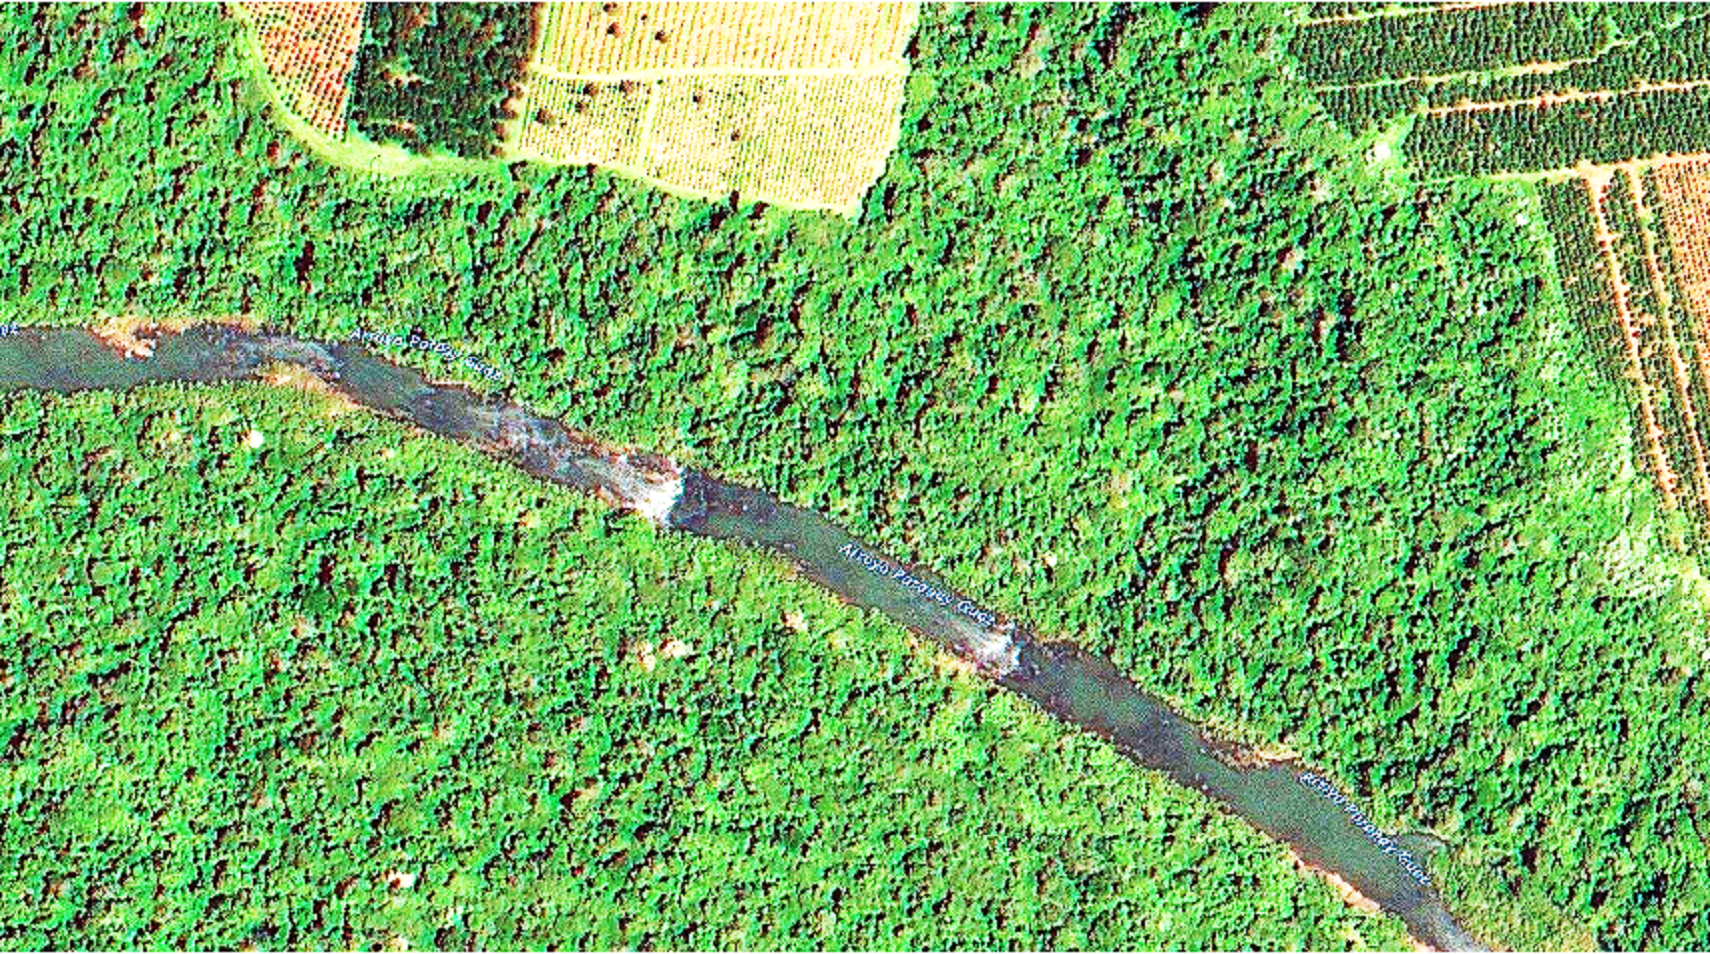
\includegraphics[width=0.5\textwidth]{Imagenes/Homomorfico/Paranai1eq.png}
     \hfill
     \caption{Imagen aérea (satelital) de una porción de selva nativa y terrenos cultivados junto al arroyo Paranay }
    %\label{Paranay1}
\end{figure}

\begin{figure}
    \includegraphics[width=.3\textwidth]{Imagenes/Homomorfico/Paranai1_bin.png}\hfill
    \includegraphics[width=.3\textwidth]{Imagenes/Homomorfico/Paranai1_masked_10.png}\hfill
    \includegraphics[width=.3\textwidth]{Imagenes/Homomorfico/Paranai1_masked_15.png}\hfill
    \\[\smallskipamount]
    \includegraphics[width=.3\textwidth]{Imagenes/Homomorfico/Paranai1_masked_20.png}\hfill
    \includegraphics[width=.3\textwidth]{Imagenes/Homomorfico/Paranai1_masked_25.png}\hfill
    \includegraphics[width=.3\textwidth]{Imagenes/Homomorfico/Paranai1_masked_30.png}\hfill
    
    \caption{Máscara binaria, sombras seleccionadas con ventana de 10, 15, 20, 25 y 30 píxeles}\label{fig:paranai1}
\end{figure}

\begin{figure}[h!]
    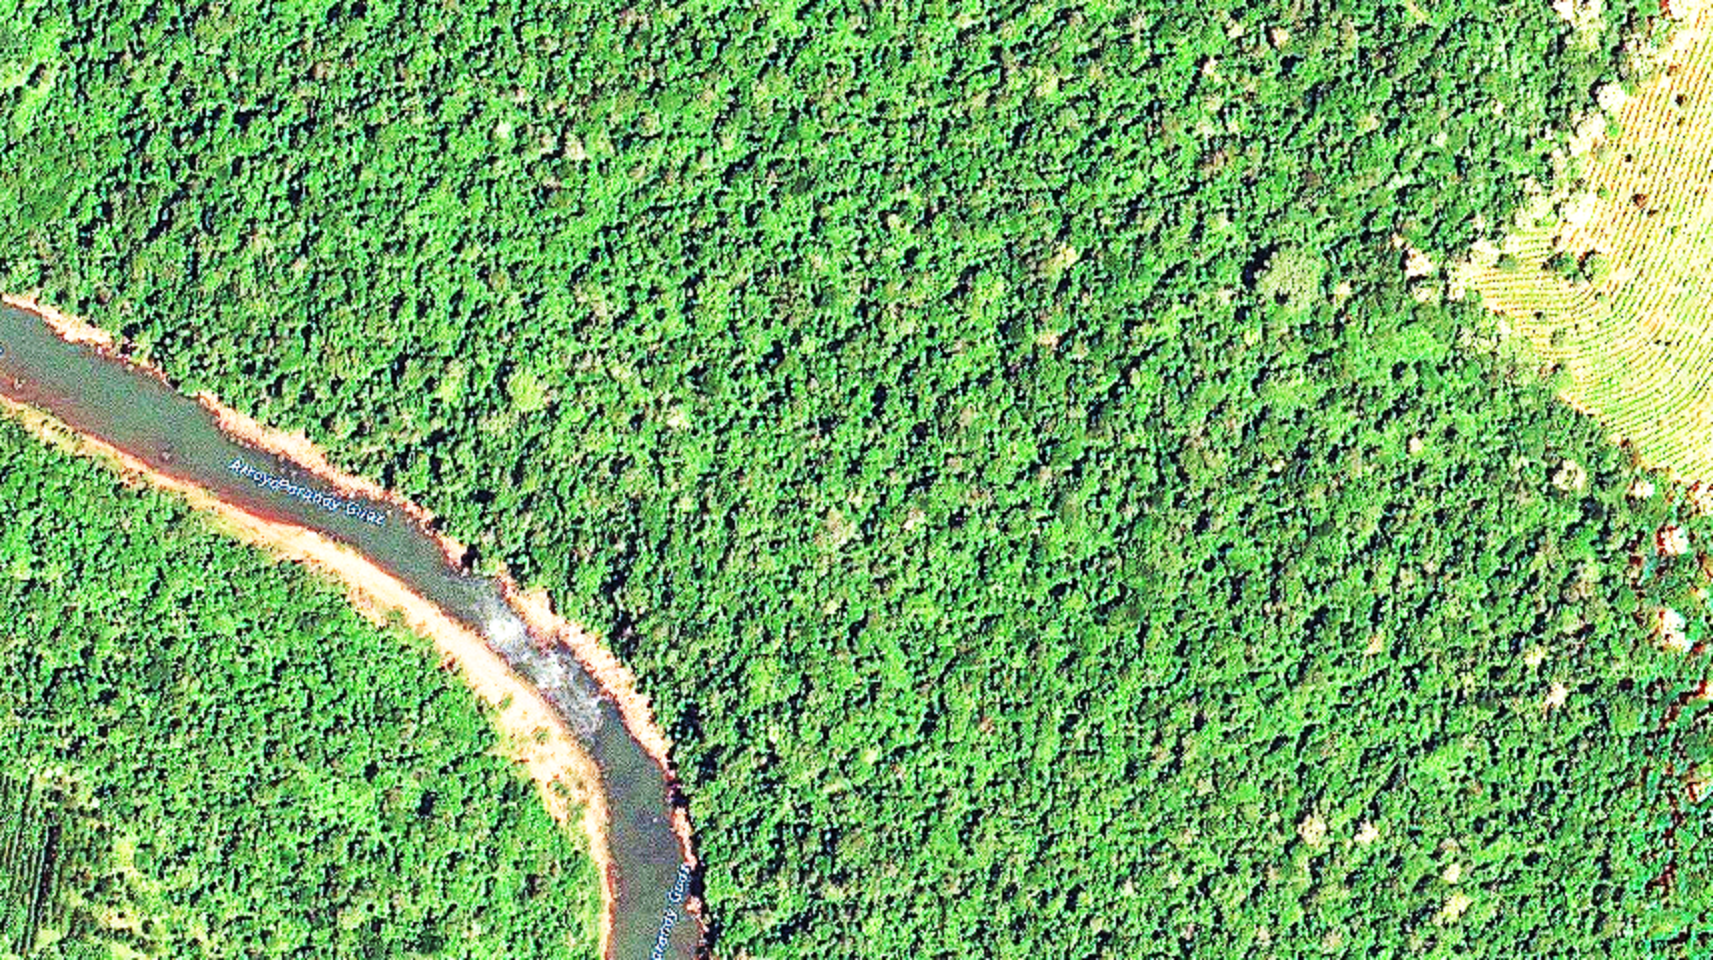
\includegraphics[width=0.5\textwidth]{Imagenes/Homomorfico/Paranai2eq.png}
     \hfill
     \caption{Imagen aérea (satelital) de una porción de selva nativa y terrenos cultivados junto al arroyo Paranay}
    %\label{Paranay2}
\end{figure}

\begin{figure}
    \includegraphics[width=.3\textwidth]{Imagenes/Homomorfico/Paranai2_bin.png}\hfill
    \includegraphics[width=.3\textwidth]{Imagenes/Homomorfico/Paranai2_masked_10.png}\hfill
    \includegraphics[width=.3\textwidth]{Imagenes/Homomorfico/Paranai2_masked_15.png}\hfill
    \\[\smallskipamount]
    \includegraphics[width=.3\textwidth]{Imagenes/Homomorfico/Paranai2_masked_20.png}\hfill
    \includegraphics[width=.3\textwidth]{Imagenes/Homomorfico/Paranai2_masked_25.png}\hfill
    \includegraphics[width=.3\textwidth]{Imagenes/Homomorfico/Paranai2_masked_30.png}\hfill
    
    \caption{Máscara binaria, sombras seleccionadas con ventana de 10, 15, 20, 25 y 30 píxeles}\label{fig:Paranai2}
\end{figure}

\begin{figure}[h!]
    \includegraphics[width=0.5\textwidth]{Imagenes/Homomorfico/PNI1gris.jpg}
     \hfill
     \caption{Imagen aérea (satelital) Parque Nacional Iguazú, en escala de grises}
    %\label{PNI1}
\end{figure}



\begin{figure}[h!]
    \includegraphics[width=0.5\textwidth]{Imagenes/Homomorfico/PNI2_original.jpg}
     \hfill
     \caption{Imagen aérea (satelital) Parque Nacional Iguazú, en RGB}
    %\label{PNI2}
\end{figure}

\begin{figure}
    \includegraphics[width=.3\textwidth]{Imagenes/Homomorfico/PNI2_bin.png}\hfill
    \includegraphics[width=.3\textwidth]{Imagenes/Homomorfico/PNI2_masked_10.png}\hfill
    \includegraphics[width=.3\textwidth]{Imagenes/Homomorfico/PNI2_masked_15.png}\hfill
    \\[\smallskipamount]
    \includegraphics[width=.3\textwidth]{Imagenes/Homomorfico/PNI2_masked_20.png}\hfill
    \includegraphics[width=.3\textwidth]{Imagenes/Homomorfico/PNI2_masked_25.png}\hfill
    \includegraphics[width=.3\textwidth]{Imagenes/Homomorfico/PNI2_masked_30.png}\hfill
    
    \caption{Máscara binaria, sombras seleccionadas con ventana de 10, 15, 20, 25 y 30 píxeles}\label{fig:Iguazu2}
\end{figure}

\begin{figure}[h!]
    \includegraphics[width=0.5\textwidth]{Imagenes/Homomorfico/PNI_03.jpg}
     \hfill
     \caption{Imagen aérea (satelital) Parque Nacional Iguazú, en RGB}
    %  \label{PNI3}
\end{figure}


\begin{figure}[h!]
    \includegraphics[width=0.5\textwidth]{Imagenes/Homomorfico/PS1_original.jpg}
     \hfill
     \caption{Imagen aérea (satelital) Parque de la Sierra, en RGB}
    %  \label{PS1}
\end{figure}

\begin{figure}
    \includegraphics[width=.3\textwidth]{Imagenes/Homomorfico/PS1_bin.png}\hfill
    \includegraphics[width=.3\textwidth]{Imagenes/Homomorfico/PS1_masked_10.png}\hfill
    \includegraphics[width=.3\textwidth]{Imagenes/Homomorfico/PS1_masked_15.png}\hfill
    \\[\smallskipamount]
    \includegraphics[width=.3\textwidth]{Imagenes/Homomorfico/PS1_masked_20.png}\hfill
    \includegraphics[width=.3\textwidth]{Imagenes/Homomorfico/PS1_masked_25.png}\hfill
    \includegraphics[width=.3\textwidth]{Imagenes/Homomorfico/PS1_masked_30.png}\hfill
    
    \caption{Máscara binaria, sombras seleccionadas con ventana de 10, 15, 20, 25 y 30 píxeles}\label{fig:Parque de la Sierra 1}
\end{figure}

\begin{figure}[h!]
    \includegraphics[width=0.5\textwidth]{Imagenes/Homomorfico/YB1.jpg}
     \hfill
     \caption{Imagen aérea (satelital) Biósfera Yaboty, en RGB}
    %  \label{YB1}
\end{figure}

\begin{figure}
    \includegraphics[width=.3\textwidth]{Imagenes/Homomorfico/YB1_bin.png}\hfill
    \includegraphics[width=.3\textwidth]{Imagenes/Homomorfico/YB1_masked_10.png}\hfill
    \includegraphics[width=.3\textwidth]{Imagenes/Homomorfico/YB1_masked_15.png}\hfill
    \\[\smallskipamount]
    \includegraphics[width=.3\textwidth]{Imagenes/Homomorfico/YB1_masked_20.png}\hfill
    \includegraphics[width=.3\textwidth]{Imagenes/Homomorfico/YB1_masked_25.png}\hfill
    \includegraphics[width=.3\textwidth]{Imagenes/Homomorfico/YB1_masked_30.png}\hfill
    
    \caption{Máscara binaria, sombras seleccionadas con ventana de 10, 15, 20, 25 y 30 píxeles}\label{fig:Yaboty1}
\end{figure}

\begin{figure}[h!]
    \includegraphics[width=0.5\textwidth]{Imagenes/Homomorfico/YB2.jpg}
     \hfill
     \caption{Imagen aérea (satelital) Biósfera Yaboty, en RGB}
    %  \label{YB2}
\end{figure}

\begin{figure}
    \includegraphics[width=.3\textwidth]{Imagenes/Homomorfico/YB2_bin.png}\hfill
    \includegraphics[width=.3\textwidth]{Imagenes/Homomorfico/YB2_masked_10.png}\hfill
    \includegraphics[width=.3\textwidth]{Imagenes/Homomorfico/YB2_masked_15.png}\hfill
    \\[\smallskipamount]
    \includegraphics[width=.3\textwidth]{Imagenes/Homomorfico/YB2_masked_20.png}\hfill
    \includegraphics[width=.3\textwidth]{Imagenes/Homomorfico/YB2_masked_25.png}\hfill
    \includegraphics[width=.3\textwidth]{Imagenes/Homomorfico/YB2_masked_30.png}\hfill
    
    \caption{Máscara binaria, sombras seleccionadas con ventana de 10, 15, 20, 25 y 30 píxeles}\label{fig:Yaboty2}
\end{figure}

\begin{figure}[h!]
    \includegraphics[width=0.5\textwidth]{Imagenes/Homomorfico/ST1_gris.png}
     \hfill
     \caption{Imagen aérea (satelital) reserva privada Sombra de Toro, en escala de grises}
    %  \label{ST1}
\end{figure}

\begin{figure}
    \includegraphics[width=.3\textwidth]{Imagenes/Homomorfico/ST1_bin.png}\hfill
    \includegraphics[width=.3\textwidth]{Imagenes/Homomorfico/ST1_masked_10.png}\hfill
    \includegraphics[width=.3\textwidth]{Imagenes/Homomorfico/ST1_masked_15.png}\hfill
    \\[\smallskipamount]
    \includegraphics[width=.3\textwidth]{Imagenes/Homomorfico/ST1_masked_20.png}\hfill
    \includegraphics[width=.3\textwidth]{Imagenes/Homomorfico/ST1_masked_25.png}\hfill
    \includegraphics[width=.3\textwidth]{Imagenes/Homomorfico/ST1_masked_30.png}\hfill
    
    \caption{Máscara binaria, sombras seleccionadas con ventana de 10, 15, 20, 25 y 30 píxeles}\label{fig:Storo1}
\end{figure}

\begin{figure}[h!]
    \includegraphics[width=0.5\textwidth]{Imagenes/Homomorfico/ST2.png}
     \hfill
     \caption{Imagen aérea (satelital) reserva privada Sombra de Toro, en RGB}
    %  \label{ST2}
\end{figure}

\begin{figure}
    \includegraphics[width=.3\textwidth]{Imagenes/Homomorfico/ST2_bin.png}\hfill
    \includegraphics[width=.3\textwidth]{Imagenes/Homomorfico/ST2_masked_10.png}\hfill
    \includegraphics[width=.3\textwidth]{Imagenes/Homomorfico/ST2_masked_15.png}\hfill
    \\[\smallskipamount]
    \includegraphics[width=.3\textwidth]{Imagenes/Homomorfico/ST2_masked_20.png}\hfill
    \includegraphics[width=.3\textwidth]{Imagenes/Homomorfico/ST2_masked_25.png}\hfill
    \includegraphics[width=.3\textwidth]{Imagenes/Homomorfico/ST2_masked_30.png}\hfill
    
    \caption{Máscara binaria, sombras seleccionadas con ventana de 10, 15, 20, 25 y 30 píxeles}\label{fig:Storo2}
\end{figure}


\chapter{Imágenes procesadas por método morfológico} \label{anexo_morfo}
  %%Anexo con imágenes analizadas con algoritmo de procesamiento homomórfico

\begin{figure}[h!]
    \includegraphics[width=0.5\textwidth]{Imagenes/Homomorfico/Paranai1eq.png}
     \hfill
     \caption{Imagen aérea (satelital) de una porción de selva nativa y terrenos cultivados junto al arroyo Paranay }
    %\label{Paranay1}
\end{figure}

\begin{figure}
    \includegraphics[width=.3\textwidth]{Imagenes/Homomorfico/Paranai1_bin.png}\hfill
    \includegraphics[width=.3\textwidth]{Imagenes/Homomorfico/Paranai1_masked_10.png}\hfill
    \includegraphics[width=.3\textwidth]{Imagenes/Homomorfico/Paranai1_masked_15.png}\hfill
    \\[\smallskipamount]
    \includegraphics[width=.3\textwidth]{Imagenes/Homomorfico/Paranai1_masked_20.png}\hfill
    \includegraphics[width=.3\textwidth]{Imagenes/Homomorfico/Paranai1_masked_25.png}\hfill
    \includegraphics[width=.3\textwidth]{Imagenes/Homomorfico/Paranai1_masked_30.png}\hfill
    
    \caption{Máscara binaria, sombras seleccionadas con ventana de 10, 15, 20, 25 y 30 píxeles}\label{fig:paranai1}
\end{figure}

\begin{figure}[h!]
    \includegraphics[width=0.5\textwidth]{Imagenes/Homomorfico/Paranai2eq.png}
     \hfill
     \caption{Imagen aérea (satelital) de una porción de selva nativa y terrenos cultivados junto al arroyo Paranay}
    %\label{Paranay2}
\end{figure}

\begin{figure}
    \includegraphics[width=.3\textwidth]{Imagenes/Homomorfico/Paranai2_bin.png}\hfill
    \includegraphics[width=.3\textwidth]{Imagenes/Homomorfico/Paranai2_masked_10.png}\hfill
    \includegraphics[width=.3\textwidth]{Imagenes/Homomorfico/Paranai2_masked_15.png}\hfill
    \\[\smallskipamount]
    \includegraphics[width=.3\textwidth]{Imagenes/Homomorfico/Paranai2_masked_20.png}\hfill
    \includegraphics[width=.3\textwidth]{Imagenes/Homomorfico/Paranai2_masked_25.png}\hfill
    \includegraphics[width=.3\textwidth]{Imagenes/Homomorfico/Paranai2_masked_30.png}\hfill
    
    \caption{Máscara binaria, sombras seleccionadas con ventana de 10, 15, 20, 25 y 30 píxeles}\label{fig:Paranai2}
\end{figure}

\begin{figure}[h!]
    \includegraphics[width=0.5\textwidth]{Imagenes/Homomorfico/PNI1gris.jpg}
     \hfill
     \caption{Imagen aérea (satelital) Parque Nacional Iguazú, en escala de grises}
    %\label{PNI1}
\end{figure}



\begin{figure}[h!]
    \includegraphics[width=0.5\textwidth]{Imagenes/Homomorfico/PNI2_original.jpg}
     \hfill
     \caption{Imagen aérea (satelital) Parque Nacional Iguazú, en RGB}
    %\label{PNI2}
\end{figure}

\begin{figure}
    \includegraphics[width=.3\textwidth]{Imagenes/Homomorfico/PNI2_bin.png}\hfill
    \includegraphics[width=.3\textwidth]{Imagenes/Homomorfico/PNI2_masked_10.png}\hfill
    \includegraphics[width=.3\textwidth]{Imagenes/Homomorfico/PNI2_masked_15.png}\hfill
    \\[\smallskipamount]
    \includegraphics[width=.3\textwidth]{Imagenes/Homomorfico/PNI2_masked_20.png}\hfill
    \includegraphics[width=.3\textwidth]{Imagenes/Homomorfico/PNI2_masked_25.png}\hfill
    \includegraphics[width=.3\textwidth]{Imagenes/Homomorfico/PNI2_masked_30.png}\hfill
    
    \caption{Máscara binaria, sombras seleccionadas con ventana de 10, 15, 20, 25 y 30 píxeles}\label{fig:Iguazu2}
\end{figure}

\begin{figure}[h!]
    \includegraphics[width=0.5\textwidth]{Imagenes/Homomorfico/PNI_03.jpg}
     \hfill
     \caption{Imagen aérea (satelital) Parque Nacional Iguazú, en RGB}
    %  \label{PNI3}
\end{figure}


\begin{figure}[h!]
    \includegraphics[width=0.5\textwidth]{Imagenes/Homomorfico/PS1_original.jpg}
     \hfill
     \caption{Imagen aérea (satelital) Parque de la Sierra, en RGB}
    %  \label{PS1}
\end{figure}

\begin{figure}
    \includegraphics[width=.3\textwidth]{Imagenes/Homomorfico/PS1_bin.png}\hfill
    \includegraphics[width=.3\textwidth]{Imagenes/Homomorfico/PS1_masked_10.png}\hfill
    \includegraphics[width=.3\textwidth]{Imagenes/Homomorfico/PS1_masked_15.png}\hfill
    \\[\smallskipamount]
    \includegraphics[width=.3\textwidth]{Imagenes/Homomorfico/PS1_masked_20.png}\hfill
    \includegraphics[width=.3\textwidth]{Imagenes/Homomorfico/PS1_masked_25.png}\hfill
    \includegraphics[width=.3\textwidth]{Imagenes/Homomorfico/PS1_masked_30.png}\hfill
    
    \caption{Máscara binaria, sombras seleccionadas con ventana de 10, 15, 20, 25 y 30 píxeles}\label{fig:Parque de la Sierra 1}
\end{figure}

\begin{figure}[h!]
    \includegraphics[width=0.5\textwidth]{Imagenes/Homomorfico/YB1.jpg}
     \hfill
     \caption{Imagen aérea (satelital) Biósfera Yaboty, en RGB}
    %  \label{YB1}
\end{figure}

\begin{figure}
    \includegraphics[width=.3\textwidth]{Imagenes/Homomorfico/YB1_bin.png}\hfill
    \includegraphics[width=.3\textwidth]{Imagenes/Homomorfico/YB1_masked_10.png}\hfill
    \includegraphics[width=.3\textwidth]{Imagenes/Homomorfico/YB1_masked_15.png}\hfill
    \\[\smallskipamount]
    \includegraphics[width=.3\textwidth]{Imagenes/Homomorfico/YB1_masked_20.png}\hfill
    \includegraphics[width=.3\textwidth]{Imagenes/Homomorfico/YB1_masked_25.png}\hfill
    \includegraphics[width=.3\textwidth]{Imagenes/Homomorfico/YB1_masked_30.png}\hfill
    
    \caption{Máscara binaria, sombras seleccionadas con ventana de 10, 15, 20, 25 y 30 píxeles}\label{fig:Yaboty1}
\end{figure}

\begin{figure}[h!]
    \includegraphics[width=0.5\textwidth]{Imagenes/Homomorfico/YB2.jpg}
     \hfill
     \caption{Imagen aérea (satelital) Biósfera Yaboty, en RGB}
    %  \label{YB2}
\end{figure}

\begin{figure}
    \includegraphics[width=.3\textwidth]{Imagenes/Homomorfico/YB2_bin.png}\hfill
    \includegraphics[width=.3\textwidth]{Imagenes/Homomorfico/YB2_masked_10.png}\hfill
    \includegraphics[width=.3\textwidth]{Imagenes/Homomorfico/YB2_masked_15.png}\hfill
    \\[\smallskipamount]
    \includegraphics[width=.3\textwidth]{Imagenes/Homomorfico/YB2_masked_20.png}\hfill
    \includegraphics[width=.3\textwidth]{Imagenes/Homomorfico/YB2_masked_25.png}\hfill
    \includegraphics[width=.3\textwidth]{Imagenes/Homomorfico/YB2_masked_30.png}\hfill
    
    \caption{Máscara binaria, sombras seleccionadas con ventana de 10, 15, 20, 25 y 30 píxeles}\label{fig:Yaboty2}
\end{figure}

\begin{figure}[h!]
    \includegraphics[width=0.5\textwidth]{Imagenes/Homomorfico/ST1_gris.png}
     \hfill
     \caption{Imagen aérea (satelital) reserva privada Sombra de Toro, en escala de grises}
    %  \label{ST1}
\end{figure}

\begin{figure}
    \includegraphics[width=.3\textwidth]{Imagenes/Homomorfico/ST1_bin.png}\hfill
    \includegraphics[width=.3\textwidth]{Imagenes/Homomorfico/ST1_masked_10.png}\hfill
    \includegraphics[width=.3\textwidth]{Imagenes/Homomorfico/ST1_masked_15.png}\hfill
    \\[\smallskipamount]
    \includegraphics[width=.3\textwidth]{Imagenes/Homomorfico/ST1_masked_20.png}\hfill
    \includegraphics[width=.3\textwidth]{Imagenes/Homomorfico/ST1_masked_25.png}\hfill
    \includegraphics[width=.3\textwidth]{Imagenes/Homomorfico/ST1_masked_30.png}\hfill
    
    \caption{Máscara binaria, sombras seleccionadas con ventana de 10, 15, 20, 25 y 30 píxeles}\label{fig:Storo1}
\end{figure}

\begin{figure}[h!]
    \includegraphics[width=0.5\textwidth]{Imagenes/Homomorfico/ST2.png}
     \hfill
     \caption{Imagen aérea (satelital) reserva privada Sombra de Toro, en RGB}
    %  \label{ST2}
\end{figure}

\begin{figure}
    \includegraphics[width=.3\textwidth]{Imagenes/Homomorfico/ST2_bin.png}\hfill
    \includegraphics[width=.3\textwidth]{Imagenes/Homomorfico/ST2_masked_10.png}\hfill
    \includegraphics[width=.3\textwidth]{Imagenes/Homomorfico/ST2_masked_15.png}\hfill
    \\[\smallskipamount]
    \includegraphics[width=.3\textwidth]{Imagenes/Homomorfico/ST2_masked_20.png}\hfill
    \includegraphics[width=.3\textwidth]{Imagenes/Homomorfico/ST2_masked_25.png}\hfill
    \includegraphics[width=.3\textwidth]{Imagenes/Homomorfico/ST2_masked_30.png}\hfill
    
    \caption{Máscara binaria, sombras seleccionadas con ventana de 10, 15, 20, 25 y 30 píxeles}\label{fig:Storo2}
\end{figure}


 \chapter{Imágenes procesadas por índice invariante de color} \label{anexo_IIC}
 %\begin{figure}
    \includegraphics[width=.3\textwidth]{Imagenes/IIC/p60/BR/180a.jpg}\hfill
    \includegraphics[width=.3\textwidth]{Imagenes/IIC/p60/BG/180a.jpg}\hfill
    \includegraphics[width=.3\textwidth]{Imagenes/IIC/p60/GR/180a.jpg}\hfill 
    \\[\smallskipamount]
    \includegraphics[width=.3\textwidth]{Imagenes/IIC/p70/BG/180a.jpg}\hfill
    \includegraphics[width=.3\textwidth]{Imagenes/IIC/p70/BG/180a.jpg}\hfill
    \includegraphics[width=.3\textwidth]{Imagenes/IIC/p70/GR/180a.jpg}\hfill
    \\[\smallskipamount]
    \includegraphics[width=.3\textwidth]{Imagenes/IIC/p80/BR/180a.jpg}\hfill
    \includegraphics[width=.3\textwidth]{Imagenes/IIC/p80/BG/180a.jpg}\hfill
    \includegraphics[width=.3\textwidth]{Imagenes/IIC/p80/GR/180a.jpg}\hfill
    \\[\smallskipamount]
    \includegraphics[width=.3\textwidth]{Imagenes/IIC/p85/BR/180a.jpg}\hfill
    \includegraphics[width=.3\textwidth]{Imagenes/IIC/p85/BG/180a.jpg}\hfill
    \includegraphics[width=.3\textwidth]{Imagenes/IIC/p85/GR/180a.jpg}\hfill
    \\[\smallskipamount]
    \includegraphics[width=.3\textwidth]{Imagenes/IIC/p90/BR/180a.jpg}\hfill
    \includegraphics[width=.3\textwidth]{Imagenes/IIC/p90/BG/180a.jpg}\hfill
    \includegraphics[width=.3\textwidth]{Imagenes/IIC/p90/GR/180a.jpg}\hfill
    
    \caption{Selección automática (en azul) vs manual (en rojo) de una imagen con diferentes combinaciones de canales y percentiles}
\end{figure}\label{dji180}

\begin{figure}
    \includegraphics[width=.3\textwidth]{Imagenes/IIC/p60/BR/190a.jpg}\hfill
    \includegraphics[width=.3\textwidth]{Imagenes/IIC/p60/BG/190a.jpg}\hfill
    \includegraphics[width=.3\textwidth]{Imagenes/IIC/p60/GR/190a.jpg}\hfill
    \\[\smallskipamount]
    \includegraphics[width=.3\textwidth]{Imagenes/IIC/p70/BG/190a.jpg}\hfill
    \includegraphics[width=.3\textwidth]{Imagenes/IIC/p70/BG/190a.jpg}\hfill
    \includegraphics[width=.3\textwidth]{Imagenes/IIC/p70/GR/190a.jpg}\hfill
    \\[\smallskipamount]
    \includegraphics[width=.3\textwidth]{Imagenes/IIC/p80/BR/190a.jpg}\hfill
    \includegraphics[width=.3\textwidth]{Imagenes/IIC/p80/BG/190a.jpg}\hfill
    \includegraphics[width=.3\textwidth]{Imagenes/IIC/p80/GR/190a.jpg}\hfill
    \\[\smallskipamount]
    \includegraphics[width=.3\textwidth]{Imagenes/IIC/p85/BR/190a.jpg}\hfill
    \includegraphics[width=.3\textwidth]{Imagenes/IIC/p85/BG/190a.jpg}\hfill
    \includegraphics[width=.3\textwidth]{Imagenes/IIC/p85/GR/190a.jpg}\hfill
    \\[\smallskipamount]
    \includegraphics[width=.3\textwidth]{Imagenes/IIC/p90/BR/190a.jpg}\hfill
    \includegraphics[width=.3\textwidth]{Imagenes/IIC/p90/BG/190a.jpg}\hfill
    \includegraphics[width=.3\textwidth]{Imagenes/IIC/p90/GR/190a.jpg}\hfill
    
    \caption{Selección automática (en azul) vs manual (en rojo) de una imagen con diferentes combinaciones de canales y percentiles}
\end{figure}\label{dji190}

\begin{figure}
    \includegraphics[width=.3\textwidth]{Imagenes/IIC/p60/BR/200a.jpg}\hfill
    \includegraphics[width=.3\textwidth]{Imagenes/IIC/p60/BG/200a.jpg}\hfill
    \includegraphics[width=.3\textwidth]{Imagenes/IIC/p60/GR/200a.jpg}\hfill
    \\[\smallskipamount]
    \includegraphics[width=.3\textwidth]{Imagenes/IIC/p70/BG/200a.jpg}\hfill
    \includegraphics[width=.3\textwidth]{Imagenes/IIC/p70/BG/200a.jpg}\hfill
    \includegraphics[width=.3\textwidth]{Imagenes/IIC/p70/GR/200a.jpg}\hfill
    \\[\smallskipamount]
    \includegraphics[width=.3\textwidth]{Imagenes/IIC/p80/BR/200a.jpg}\hfill
    \includegraphics[width=.3\textwidth]{Imagenes/IIC/p80/BG/200a.jpg}\hfill
    \includegraphics[width=.3\textwidth]{Imagenes/IIC/p80/GR/200a.jpg}\hfill
    \\[\smallskipamount]
    \includegraphics[width=.3\textwidth]{Imagenes/IIC/p85/BR/200a.jpg}\hfill
    \includegraphics[width=.3\textwidth]{Imagenes/IIC/p85/BG/200a.jpg}\hfill
    \includegraphics[width=.3\textwidth]{Imagenes/IIC/p85/GR/200a.jpg}\hfill
    \\[\smallskipamount]
    \includegraphics[width=.3\textwidth]{Imagenes/IIC/p90/BR/200a.jpg}\hfill
    \includegraphics[width=.3\textwidth]{Imagenes/IIC/p90/BG/200a.jpg}\hfill
    \includegraphics[width=.3\textwidth]{Imagenes/IIC/p90/GR/200a.jpg}\hfill
    
    \caption{Selección automática (en azul) vs manual (en rojo) de una imagen con diferentes combinaciones de canales y percentiles}
\end{figure}\label{dji200}

\begin{figure}
    \includegraphics[width=.3\textwidth]{Imagenes/IIC/p60/BR/210a.jpg}\hfill
    \includegraphics[width=.3\textwidth]{Imagenes/IIC/p60/BG/210a.jpg}\hfill
    \includegraphics[width=.3\textwidth]{Imagenes/IIC/p60/GR/210a.jpg}\hfill
    \\[\smallskipamount]
    \includegraphics[width=.3\textwidth]{Imagenes/IIC/p70/BG/210a.jpg}\hfill
    \includegraphics[width=.3\textwidth]{Imagenes/IIC/p70/BG/210a.jpg}\hfill
    \includegraphics[width=.3\textwidth]{Imagenes/IIC/p70/BG/210a.jpg}\hfill
    \\[\smallskipamount]
    \includegraphics[width=.3\textwidth]{Imagenes/IIC/p80/BR/210a.jpg}\hfill
    \includegraphics[width=.3\textwidth]{Imagenes/IIC/p80/BG/210a.jpg}\hfill
    \includegraphics[width=.3\textwidth]{Imagenes/IIC/p80/GR/210a.jpg}\hfill
    \\[\smallskipamount]
    \includegraphics[width=.3\textwidth]{Imagenes/IIC/p85/BR/210a.jpg}\hfill
    \includegraphics[width=.3\textwidth]{Imagenes/IIC/p85/BG/210a.jpg}\hfill
    \includegraphics[width=.3\textwidth]{Imagenes/IIC/p85/GR/210a.jpg}\hfill
    \\[\smallskipamount]
    \includegraphics[width=.3\textwidth]{Imagenes/IIC/p90/BR/210a.jpg}\hfill
    \includegraphics[width=.3\textwidth]{Imagenes/IIC/p90/BG/210a.jpg}\hfill
    \includegraphics[width=.3\textwidth]{Imagenes/IIC/p90/GR/210a.jpg}\hfill
    
    \caption{Selección automática (en azul) vs manual (en rojo) de una imagen con diferentes combinaciones de canales y percentiles}
\end{figure}\label{dji210}

\begin{figure}
    \includegraphics[width=.3\textwidth]{Imagenes/IIC/p60/BR/220a.jpg}\hfill
    \includegraphics[width=.3\textwidth]{Imagenes/IIC/p60/BG/220a.jpg}\hfill
    \includegraphics[width=.3\textwidth]{Imagenes/IIC/p60/GR/220a.jpg}\hfill
    \\[\smallskipamount]
    \includegraphics[width=.3\textwidth]{Imagenes/IIC/p70/BR/220a.jpg}\hfill
    \includegraphics[width=.3\textwidth]{Imagenes/IIC/p70/BG/220a.jpg}\hfill
    \includegraphics[width=.3\textwidth]{Imagenes/IIC/p70/BG/220a.jpg}\hfill
    \\[\smallskipamount]
    \includegraphics[width=.3\textwidth]{Imagenes/IIC/p80/BR/220a.jpg}\hfill
    \includegraphics[width=.3\textwidth]{Imagenes/IIC/p80/BG/220a.jpg}\hfill
    \includegraphics[width=.3\textwidth]{Imagenes/IIC/p80/GR/220a.jpg}\hfill
    \\[\smallskipamount]
    \includegraphics[width=.3\textwidth]{Imagenes/IIC/p85/BR/220a.jpg}\hfill
    \includegraphics[width=.3\textwidth]{Imagenes/IIC/p85/BG/220a.jpg}\hfill
    \includegraphics[width=.3\textwidth]{Imagenes/IIC/p85/GR/220a.jpg}\hfill
    \\[\smallskipamount]
    \includegraphics[width=.3\textwidth]{Imagenes/IIC/p90/BR/220a.jpg}\hfill
    \includegraphics[width=.3\textwidth]{Imagenes/IIC/p90/BG/220a.jpg}\hfill
    \includegraphics[width=.3\textwidth]{Imagenes/IIC/p90/GR/220a.jpg}\hfill
    
    \caption{Selección automática (en azul) vs manual (en rojo) de una imagen con diferentes combinaciones de canales y percentiles}
\end{figure}\label{dji220}

\begin{figure}
    \includegraphics[width=.3\textwidth]{Imagenes/IIC/p60/BR/230a.jpg}\hfill
    \includegraphics[width=.3\textwidth]{Imagenes/IIC/p60/BG/230a.jpg}\hfill
    \includegraphics[width=.3\textwidth]{Imagenes/IIC/p60/GR/230a.jpg}\hfill
    \\[\smallskipamount]
    \includegraphics[width=.3\textwidth]{Imagenes/IIC/p70/BR/230a.jpg}\hfill
    \includegraphics[width=.3\textwidth]{Imagenes/IIC/p70/BG/230a.jpg}\hfill
    \includegraphics[width=.3\textwidth]{Imagenes/IIC/p70/BG/230a.jpg}\hfill
    \\[\smallskipamount]
    \includegraphics[width=.3\textwidth]{Imagenes/IIC/p80/BR/230a.jpg}\hfill
    \includegraphics[width=.3\textwidth]{Imagenes/IIC/p80/BG/230a.jpg}\hfill
    \includegraphics[width=.3\textwidth]{Imagenes/IIC/p80/GR/230a.jpg}\hfill
    \\[\smallskipamount]
    \includegraphics[width=.3\textwidth]{Imagenes/IIC/p85/BR/230a.jpg}\hfill
    \includegraphics[width=.3\textwidth]{Imagenes/IIC/p85/BG/230a.jpg}\hfill
    \includegraphics[width=.3\textwidth]{Imagenes/IIC/p85/GR/230a.jpg}\hfill
    \\[\smallskipamount]
    \includegraphics[width=.3\textwidth]{Imagenes/IIC/p90/BR/230a.jpg}\hfill
    \includegraphics[width=.3\textwidth]{Imagenes/IIC/p90/BG/230a.jpg}\hfill
    \includegraphics[width=.3\textwidth]{Imagenes/IIC/p90/GR/230a.jpg}\hfill
    
    \caption{Selección automática (en azul) vs manual (en rojo) de una imagen con diferentes combinaciones de canales y percentiles}
\end{figure}\label{dji230}

\begin{figure}
    \includegraphics[width=.3\textwidth]{Imagenes/IIC/p60/BR/240a.jpg}\hfill
    \includegraphics[width=.3\textwidth]{Imagenes/IIC/p60/BG/240a.jpg}\hfill
    \includegraphics[width=.3\textwidth]{Imagenes/IIC/p60/GR/240a.jpg}\hfill
    \\[\smallskipamount]
    \includegraphics[width=.3\textwidth]{Imagenes/IIC/p70/BG/240a.jpg}\hfill
    \includegraphics[width=.3\textwidth]{Imagenes/IIC/p70/BG/240a.jpg}\hfill
    \includegraphics[width=.3\textwidth]{Imagenes/IIC/p70/BG/240a.jpg}\hfill
    \\[\smallskipamount]
    \includegraphics[width=.3\textwidth]{Imagenes/IIC/p80/BR/240a.jpg}\hfill
    \includegraphics[width=.3\textwidth]{Imagenes/IIC/p80/BG/240a.jpg}\hfill
    \includegraphics[width=.3\textwidth]{Imagenes/IIC/p80/GR/240a.jpg}\hfill
    \\[\smallskipamount]
    \includegraphics[width=.3\textwidth]{Imagenes/IIC/p85/BR/240a.jpg}\hfill
    \includegraphics[width=.3\textwidth]{Imagenes/IIC/p85/BG/240a.jpg}\hfill
    \includegraphics[width=.3\textwidth]{Imagenes/IIC/p85/GR/240a.jpg}\hfill
    \\[\smallskipamount]
    \includegraphics[width=.3\textwidth]{Imagenes/IIC/p90/BR/240a.jpg}\hfill
    \includegraphics[width=.3\textwidth]{Imagenes/IIC/p90/BG/240a.jpg}\hfill
    \includegraphics[width=.3\textwidth]{Imagenes/IIC/p90/GR/240a.jpg}\hfill
    
    \caption{Selección automática (en azul) vs manual (en rojo) de una imagen con diferentes combinaciones de canales y percentiles}
\end{figure}\label{dji240}

\begin{figure}
    \includegraphics[width=.3\textwidth]{Imagenes/IIC/p60/BR/250a.jpg}\hfill
    \includegraphics[width=.3\textwidth]{Imagenes/IIC/p60/BG/250a.jpg}\hfill
    \includegraphics[width=.3\textwidth]{Imagenes/IIC/p60/GR/250a.jpg}\hfill
    \\[\smallskipamount]
    \includegraphics[width=.3\textwidth]{Imagenes/IIC/p70/BR/250a.jpg}\hfill
    \includegraphics[width=.3\textwidth]{Imagenes/IIC/p70/BG/250a.jpg}\hfill
    \includegraphics[width=.3\textwidth]{Imagenes/IIC/p70/GR/250a.jpg}\hfill
    \\[\smallskipamount]
    \includegraphics[width=.3\textwidth]{Imagenes/IIC/p80/BG/250a.jpg}\hfill
    \includegraphics[width=.3\textwidth]{Imagenes/IIC/p80/BG/250a.jpg}\hfill
    \includegraphics[width=.3\textwidth]{Imagenes/IIC/p80/GR/250a.jpg}\hfill
    \\[\smallskipamount]
    \includegraphics[width=.3\textwidth]{Imagenes/IIC/p85/BR/250a.jpg}\hfill
    \includegraphics[width=.3\textwidth]{Imagenes/IIC/p85/BG/250a.jpg}\hfill
    \includegraphics[width=.3\textwidth]{Imagenes/IIC/p85/GR/250a.jpg}\hfill
    \\[\smallskipamount]
    \includegraphics[width=.3\textwidth]{Imagenes/IIC/p90/BR/250a.jpg}\hfill
    \includegraphics[width=.3\textwidth]{Imagenes/IIC/p90/BG/250a.jpg}\hfill
    \includegraphics[width=.3\textwidth]{Imagenes/IIC/p90/GR/250a.jpg}\hfill
    
    \caption{Selección automática (en azul) vs manual (en rojo) de una imagen con diferentes combinaciones de canales y percentiles}
\end{figure}\label{dji250}

\begin{figure}
    \includegraphics[width=.3\textwidth]{Imagenes/IIC/p60/BR/260a.jpg}\hfill
    \includegraphics[width=.3\textwidth]{Imagenes/IIC/p60/BG/260a.jpg}\hfill
    \includegraphics[width=.3\textwidth]{Imagenes/IIC/p60/GR/260a.jpg}\hfill
    \\[\smallskipamount]
    \includegraphics[width=.3\textwidth]{Imagenes/IIC/p80/BR/260a.jpg}\hfill
    \includegraphics[width=.3\textwidth]{Imagenes/IIC/p80/BG/260a.jpg}\hfill
    \includegraphics[width=.3\textwidth]{Imagenes/IIC/p80/GR/260a.jpg}\hfill
    \\[\smallskipamount]
    \includegraphics[width=.3\textwidth]{Imagenes/IIC/p85/BR/260a.jpg}\hfill
    \includegraphics[width=.3\textwidth]{Imagenes/IIC/p85/BG/260a.jpg}\hfill
    \includegraphics[width=.3\textwidth]{Imagenes/IIC/p85/GR/260a.jpg}\hfill
    \\[\smallskipamount]
    \includegraphics[width=.3\textwidth]{Imagenes/IIC/p90/BR/260a.jpg}\hfill
    \includegraphics[width=.3\textwidth]{Imagenes/IIC/p90/BG/260a.jpg}\hfill
    \includegraphics[width=.3\textwidth]{Imagenes/IIC/p90/GR/260a.jpg}\hfill
    
    \caption{Selección automática (en azul) vs manual (en rojo) de una imagen con diferentes combinaciones de canales y percentiles}
\end{figure}\label{dji260}

\begin{figure}
    \includegraphics[width=.3\textwidth]{Imagenes/IIC/p60/BR/270a.jpg}\hfill
    \includegraphics[width=.3\textwidth]{Imagenes/IIC/p60/BG/270a.jpg}\hfill
    \includegraphics[width=.3\textwidth]{Imagenes/IIC/p60/GR/270a.jpg}\hfill
    \\[\smallskipamount]
    \includegraphics[width=.3\textwidth]{Imagenes/IIC/p70/BR/270a.jpg}\hfill
    \includegraphics[width=.3\textwidth]{Imagenes/IIC/p70/BG/270a.jpg}\hfill
    \includegraphics[width=.3\textwidth]{Imagenes/IIC/p70/GR/270a.jpg}\hfill
    \\[\smallskipamount]
    \includegraphics[width=.3\textwidth]{Imagenes/IIC/p80/BR/270a.jpg}\hfill
    \includegraphics[width=.3\textwidth]{Imagenes/IIC/p80/BG/270a.jpg}\hfill
    \includegraphics[width=.3\textwidth]{Imagenes/IIC/p80/GR/270a.jpg}\hfill
    \\[\smallskipamount]
    \includegraphics[width=.3\textwidth]{Imagenes/IIC/p85/BR/270a.jpg}\hfill
    \includegraphics[width=.3\textwidth]{Imagenes/IIC/p85/BG/270a.jpg}\hfill
    \includegraphics[width=.3\textwidth]{Imagenes/IIC/p85/GR/270a.jpg}\hfill
    \\[\smallskipamount]
    \includegraphics[width=.3\textwidth]{Imagenes/IIC/p90/BR/270a.jpg}\hfill
    \includegraphics[width=.3\textwidth]{Imagenes/IIC/p90/BG/270a.jpg}\hfill
    \includegraphics[width=.3\textwidth]{Imagenes/IIC/p90/GR/270a.jpg}\hfill
    
    \caption{Selección automática (en azul) vs manual (en rojo) de una imagen con diferentes combinaciones de canales y percentiles}
\end{figure}\label{dji270}

\begin{figure}
    \includegraphics[width=.3\textwidth]{Imagenes/IIC/p60/BR/280a.jpg}\hfill
    \includegraphics[width=.3\textwidth]{Imagenes/IIC/p60/BG/280a.jpg}\hfill
    \includegraphics[width=.3\textwidth]{Imagenes/IIC/p60/GR/280a.jpg}\hfill
    \\[\smallskipamount]
    \includegraphics[width=.3\textwidth]{Imagenes/IIC/p80/BR/280a.jpg}\hfill
    \includegraphics[width=.3\textwidth]{Imagenes/IIC/p80/BG/280a.jpg}\hfill
    \includegraphics[width=.3\textwidth]{Imagenes/IIC/p80/GR/280a.jpg}\hfill
    \\[\smallskipamount]
    \includegraphics[width=.3\textwidth]{Imagenes/IIC/p85/BR/280a.jpg}\hfill
    \includegraphics[width=.3\textwidth]{Imagenes/IIC/p85/BG/280a.jpg}\hfill
    \includegraphics[width=.3\textwidth]{Imagenes/IIC/p85/GR/280a.jpg}\hfill
    \\[\smallskipamount]
    \includegraphics[width=.3\textwidth]{Imagenes/IIC/p90/BR/280a.jpg}\hfill
    \includegraphics[width=.3\textwidth]{Imagenes/IIC/p90/BG/280a.jpg}\hfill
    \includegraphics[width=.3\textwidth]{Imagenes/IIC/p90/GR/280a.jpg}\hfill
    
    \caption{Selección automática (en azul) vs manual (en rojo) de una imagen con diferentes combinaciones de canales y percentiles}
\end{figure}\label{dji280}

\begin{figure}
    \includegraphics[width=.3\textwidth]{Imagenes/IIC/p60/BR/290a.jpg}\hfill
    \includegraphics[width=.3\textwidth]{Imagenes/IIC/p60/BG/290a.jpg}\hfill
    \includegraphics[width=.3\textwidth]{Imagenes/IIC/p60/GR/290a.jpg}\hfill
    \\[\smallskipamount]
    \includegraphics[width=.3\textwidth]{Imagenes/IIC/p80/BR/290a.jpg}\hfill
    \includegraphics[width=.3\textwidth]{Imagenes/IIC/p80/BG/290a.jpg}\hfill
    \includegraphics[width=.3\textwidth]{Imagenes/IIC/p80/GR/290a.jpg}\hfill
    \\[\smallskipamount]
    \includegraphics[width=.3\textwidth]{Imagenes/IIC/p85/BR/290a.jpg}\hfill
    \includegraphics[width=.3\textwidth]{Imagenes/IIC/p85/BG/290a.jpg}\hfill
    \includegraphics[width=.3\textwidth]{Imagenes/IIC/p85/GR/290a.jpg}\hfill
    \\[\smallskipamount]
    \includegraphics[width=.3\textwidth]{Imagenes/IIC/p90/BR/290a.jpg}\hfill
    \includegraphics[width=.3\textwidth]{Imagenes/IIC/p90/BG/290a.jpg}\hfill
    \includegraphics[width=.3\textwidth]{Imagenes/IIC/p90/GR/290a.jpg}\hfill
    
    \caption{Selección automática (en azul) vs manual (en rojo) de una imagen con diferentes combinaciones de canales y percentiles}
\end{figure}\label{dji290}

\begin{figure}
    \includegraphics[width=.3\textwidth]{Imagenes/IIC/p60/BR/300a.jpg}\hfill
    \includegraphics[width=.3\textwidth]{Imagenes/IIC/p60/BG/300a.jpg}\hfill
    \includegraphics[width=.3\textwidth]{Imagenes/IIC/p60/GR/300a.jpg}\hfill
    \\[\smallskipamount]
    \includegraphics[width=.3\textwidth]{Imagenes/IIC/p80/BR/300a.jpg}\hfill
    \includegraphics[width=.3\textwidth]{Imagenes/IIC/p80/BG/300a.jpg}\hfill
    \includegraphics[width=.3\textwidth]{Imagenes/IIC/p80/GR/300a.jpg}\hfill
    \\[\smallskipamount]
    \includegraphics[width=.3\textwidth]{Imagenes/IIC/p85/BR/300a.jpg}\hfill
    \includegraphics[width=.3\textwidth]{Imagenes/IIC/p85/BG/300a.jpg}\hfill
    \includegraphics[width=.3\textwidth]{Imagenes/IIC/p85/GR/300a.jpg}\hfill
    \\[\smallskipamount]
    \includegraphics[width=.3\textwidth]{Imagenes/IIC/p90/BR/300a.jpg}\hfill
    \includegraphics[width=.3\textwidth]{Imagenes/IIC/p90/BG/300a.jpg}\hfill
    \includegraphics[width=.3\textwidth]{Imagenes/IIC/p90/GR/300a.jpg}\hfill
    
    \caption{Selección automática (en azul) vs manual (en rojo) de una imagen con diferentes combinaciones de canales y percentiles}
\end{figure}\label{dji300}

\begin{figure}
    \includegraphics[width=.3\textwidth]{Imagenes/IIC/p60/BR/310a.jpg}\hfill
    \includegraphics[width=.3\textwidth]{Imagenes/IIC/p60/BG/310a.jpg}\hfill
    \includegraphics[width=.3\textwidth]{Imagenes/IIC/p60/GR/310a.jpg}\hfill
    \\[\smallskipamount]
    \includegraphics[width=.3\textwidth]{Imagenes/IIC/p80/BR/310a.jpg}\hfill
    \includegraphics[width=.3\textwidth]{Imagenes/IIC/p80/BG/310a.jpg}\hfill
    \includegraphics[width=.3\textwidth]{Imagenes/IIC/p80/GR/310a.jpg}\hfill
    \\[\smallskipamount]
    \includegraphics[width=.3\textwidth]{Imagenes/IIC/p85/BR/310a.jpg}\hfill
    \includegraphics[width=.3\textwidth]{Imagenes/IIC/p85/BG/310a.jpg}\hfill
    \includegraphics[width=.3\textwidth]{Imagenes/IIC/p85/GR/310a.jpg}\hfill
    \\[\smallskipamount]
    \includegraphics[width=.3\textwidth]{Imagenes/IIC/p90/BR/310a.jpg}\hfill
    \includegraphics[width=.3\textwidth]{Imagenes/IIC/p90/BG/310a.jpg}\hfill
    \includegraphics[width=.3\textwidth]{Imagenes/IIC/p90/GR/310a.jpg}\hfill
    
    \caption{Selección automática (en azul) vs manual (en rojo) de una imagen con diferentes combinaciones de canales y percentiles}
\end{figure}\label{dji310}

\begin{figure}
    \includegraphics[width=.3\textwidth]{Imagenes/IIC/p60/BR/320a.jpg}\hfill
    \includegraphics[width=.3\textwidth]{Imagenes/IIC/p60/BG/320a.jpg}\hfill
    \includegraphics[width=.3\textwidth]{Imagenes/IIC/p60/GR/320a.jpg}\hfill
    \\[\smallskipamount]
    \includegraphics[width=.3\textwidth]{Imagenes/IIC/p80/BR/320a.jpg}\hfill
    \includegraphics[width=.3\textwidth]{Imagenes/IIC/p80/BG/320a.jpg}\hfill
    \includegraphics[width=.3\textwidth]{Imagenes/IIC/p80/GR/320a.jpg}\hfill
    \\[\smallskipamount]
    \includegraphics[width=.3\textwidth]{Imagenes/IIC/p85/BR/320a.jpg}\hfill
    \includegraphics[width=.3\textwidth]{Imagenes/IIC/p85/BG/320a.jpg}\hfill
    \includegraphics[width=.3\textwidth]{Imagenes/IIC/p85/GR/320a.jpg}\hfill
    \\[\smallskipamount]
    \includegraphics[width=.3\textwidth]{Imagenes/IIC/p90/BR/320a.jpg}\hfill
    \includegraphics[width=.3\textwidth]{Imagenes/IIC/p90/BG/320a.jpg}\hfill
    \includegraphics[width=.3\textwidth]{Imagenes/IIC/p90/GR/320a.jpg}\hfill
    
    \caption{Selección automática (en azul) vs manual (en rojo) de una imagen con diferentes combinaciones de canales y percentiles}
\end{figure}\label{dji320}

\begin{figure}
    \includegraphics[width=.3\textwidth]{Imagenes/IIC/p60/BR/330a.jpg}\hfill
    \includegraphics[width=.3\textwidth]{Imagenes/IIC/p60/BG/330a.jpg}\hfill
    \includegraphics[width=.3\textwidth]{Imagenes/IIC/p60/GR/330a.jpg}\hfill
    \\[\smallskipamount]
    \includegraphics[width=.3\textwidth]{Imagenes/IIC/p80/BR/330a.jpg}\hfill
    \includegraphics[width=.3\textwidth]{Imagenes/IIC/p80/BG/330a.jpg}\hfill
    \includegraphics[width=.3\textwidth]{Imagenes/IIC/p80/GR/330a.jpg}\hfill
    \\[\smallskipamount]
    \includegraphics[width=.3\textwidth]{Imagenes/IIC/p85/BR/330a.jpg}\hfill
    \includegraphics[width=.3\textwidth]{Imagenes/IIC/p85/BG/330a.jpg}\hfill
    \includegraphics[width=.3\textwidth]{Imagenes/IIC/p85/GR/330a.jpg}\hfill
    \\[\smallskipamount]
    \includegraphics[width=.3\textwidth]{Imagenes/IIC/p90/BR/330a.jpg}\hfill
    \includegraphics[width=.3\textwidth]{Imagenes/IIC/p90/BG/330a.jpg}\hfill
    \includegraphics[width=.3\textwidth]{Imagenes/IIC/p90/GR/330a.jpg}\hfill
    
    \caption{Selección automática (en azul) vs manual (en rojo) de una imagen con diferentes combinaciones de canales y percentiles}
\end{figure}\label{dji330}

\begin{figure}
    \includegraphics[width=.3\textwidth]{Imagenes/IIC/p60/BR/340a.jpg}\hfill
    \includegraphics[width=.3\textwidth]{Imagenes/IIC/p60/BG/340a.jpg}\hfill
    \includegraphics[width=.3\textwidth]{Imagenes/IIC/p60/GR/340a.jpg}\hfill
    \\[\smallskipamount]
    \includegraphics[width=.3\textwidth]{Imagenes/IIC/p80/BR/340a.jpg}\hfill
    \includegraphics[width=.3\textwidth]{Imagenes/IIC/p80/BG/340a.jpg}\hfill
    \includegraphics[width=.3\textwidth]{Imagenes/IIC/p80/GR/340a.jpg}\hfill
    \\[\smallskipamount]
    \includegraphics[width=.3\textwidth]{Imagenes/IIC/p85/BR/340a.jpg}\hfill
    \includegraphics[width=.3\textwidth]{Imagenes/IIC/p85/BG/340a.jpg}\hfill
    \includegraphics[width=.3\textwidth]{Imagenes/IIC/p85/GR/340a.jpg}\hfill
    \\[\smallskipamount]
    \includegraphics[width=.3\textwidth]{Imagenes/IIC/p90/BR/340a.jpg}\hfill
    \includegraphics[width=.3\textwidth]{Imagenes/IIC/p90/BG/340a.jpg}\hfill
    \includegraphics[width=.3\textwidth]{Imagenes/IIC/p90/GR/340a.jpg}\hfill
    
    \caption{Selección automática (en azul) vs manual (en rojo) de una imagen con diferentes combinaciones de canales y percentiles}
\end{figure}\label{dji340}

\begin{figure}
    \includegraphics[width=.3\textwidth]{Imagenes/IIC/p60/BR/350a.jpg}\hfill
    \includegraphics[width=.3\textwidth]{Imagenes/IIC/p60/BG/350a.jpg}\hfill
    \includegraphics[width=.3\textwidth]{Imagenes/IIC/p60/GR/350a.jpg}\hfill
    \\[\smallskipamount]
    \includegraphics[width=.3\textwidth]{Imagenes/IIC/p80/BR/350a.jpg}\hfill
    \includegraphics[width=.3\textwidth]{Imagenes/IIC/p80/BG/350a.jpg}\hfill
    \includegraphics[width=.3\textwidth]{Imagenes/IIC/p80/GR/350a.jpg}\hfill
    \\[\smallskipamount]
    \includegraphics[width=.3\textwidth]{Imagenes/IIC/p85/BR/350a.jpg}\hfill
    \includegraphics[width=.3\textwidth]{Imagenes/IIC/p85/BG/350a.jpg}\hfill
    \includegraphics[width=.3\textwidth]{Imagenes/IIC/p85/GR/350a.jpg}\hfill
    \\[\smallskipamount]
    \includegraphics[width=.3\textwidth]{Imagenes/IIC/p90/BR/350a.jpg}\hfill
    \includegraphics[width=.3\textwidth]{Imagenes/IIC/p90/BG/350a.jpg}\hfill
    \includegraphics[width=.3\textwidth]{Imagenes/IIC/p90/GR/350a.jpg}\hfill
    
    \caption{Selección automática (en azul) vs manual (en rojo) de una imagen con diferentes combinaciones de canales y percentiles}
\end{figure}\label{dji350}

\begin{figure}
    \includegraphics[width=.3\textwidth]{Imagenes/IIC/p60/BR/360a.jpg}\hfill
    \includegraphics[width=.3\textwidth]{Imagenes/IIC/p60/BG/360a.jpg}\hfill
    \includegraphics[width=.3\textwidth]{Imagenes/IIC/p60/GR/360a.jpg}\hfill
    \\[\smallskipamount]
    \includegraphics[width=.3\textwidth]{Imagenes/IIC/p80/BR/360a.jpg}\hfill
    \includegraphics[width=.3\textwidth]{Imagenes/IIC/p80/BG/360a.jpg}\hfill
    \includegraphics[width=.3\textwidth]{Imagenes/IIC/p80/GR/360a.jpg}\hfill
    \\[\smallskipamount]
    \includegraphics[width=.3\textwidth]{Imagenes/IIC/p85/BR/360a.jpg}\hfill
    \includegraphics[width=.3\textwidth]{Imagenes/IIC/p85/BG/360a.jpg}\hfill
    \includegraphics[width=.3\textwidth]{Imagenes/IIC/p85/GR/360a.jpg}\hfill
    \\[\smallskipamount]
    \includegraphics[width=.3\textwidth]{Imagenes/IIC/p90/BR/360a.jpg}\hfill
    \includegraphics[width=.3\textwidth]{Imagenes/IIC/p90/BG/360a.jpg}\hfill
    \includegraphics[width=.3\textwidth]{Imagenes/IIC/p90/GR/360a.jpg}\hfill
    
    \caption{Selección automática (en azul) vs manual (en rojo) de una imagen con diferentes combinaciones de canales y percentiles}
\end{figure}\label{dji360}
\chapter{Machine learning} 
\subsection{C3-Filtros de texturas (probados con fantomas)} %va en apéndice
Mediante el filtrado por textura puede implementarse una segmentación o clasificación en imágenes. Se hicieron varias pruebas con imágenes simuladas (cuadrados y rombos)


\chapter{Fuzzy logic} 
    Nada más que probar qué pasa...
\subsection{Machine learning (¿?)}

%●	Carátula (con el formato solicitado por el DCA que se adjunta al presente Anexo)
%●	Agradecimientos
%●	Índice
%●	Listado de Abreviaturas (en caso de que lo considere conveniente)
	


%---------------------------------------------------------------------------------------------------------------------
\printbibliography[title={Referencias}, heading=bibintoc]
\end{document}
%%%%%%%%%%%%%%%%%%%%%%%%%%%%%%%%%%%%%%%%%%%%%%%%%%%%%%%%%%%%%%%%%%%%%%%%%%%%%%%%%%%%%%%%%%%%%%%%%%%%%%%%%%%%%%%%%%%%%%
